%% ============================================================
%% MIVA-KNIGHT-RL: Complete Thesis
%% Reinforcement Learning-Driven Multimodal Robot Control
%% with Deep Q-Network, Experience Replay, and
%% Hybrid Knowledge-Augmented Generation
%% Author: Oluwakayode (Kayode) Soyinka
%% IT 581 Capstone — Concordia University of Edmonton
%% Supervisor: Dr. Baidya Saha
%% ============================================================
\documentclass[12pt,a4paper]{article}

%% ── Encoding & Fonts ────────────────────────────────────────
\usepackage[utf8]{inputenc}
\usepackage[T1]{fontenc}
\usepackage{microtype}

%% ── Page Geometry ───────────────────────────────────────────
\usepackage[margin=2.5cm,top=3cm,bottom=3cm]{geometry}

%% ── Mathematics ─────────────────────────────────────────────
\usepackage{amsmath,amssymb,amsthm,mathtools}
\usepackage{bm}

%% ── Algorithms ──────────────────────────────────────────────
\usepackage{algorithm}
\usepackage{algpseudocode}
\usepackage{algorithmicx}
\algnewcommand\algorithmicforeach{\textbf{for each}}
\algdef{S}[FOR]{ForEach}[1]{\algorithmicforeach\ #1\ \textbf{do}}
\renewcommand{\algorithmicrequire}{\textbf{Require:}}
\renewcommand{\algorithmicensure}{\textbf{Ensure:}}

%% ── TikZ & Drawing ──────────────────────────────────────────
\usepackage{tikz}
\usetikzlibrary{
  shapes.geometric, shapes.misc,
  arrows.meta, arrows,
  positioning, fit, calc,
  backgrounds, patterns,
  decorations.pathreplacing,
  decorations.markings,
  matrix, chains, shadows
}
\usepackage{pgfplots}
\pgfplotsset{compat=1.18}

%% ── Scaling & Figures ───────────────────────────────────────
\usepackage{graphicx}
\usepackage{adjustbox}
\usepackage{float}
\usepackage{caption}
\usepackage{subcaption}

%% ── Tables ──────────────────────────────────────────────────
\usepackage{booktabs}
\usepackage{tabularx}
\usepackage{longtable}
\usepackage{multirow}
\usepackage{colortbl}
\usepackage{array}

%% ── Colours ─────────────────────────────────────────────────
\usepackage[dvipsnames,svgnames,table]{xcolor}

%% ── Boxes ───────────────────────────────────────────────────
\usepackage{tcolorbox}
\tcbuselibrary{breakable,skins,theorems}

%% ── Typography ──────────────────────────────────────────────
\usepackage{setspace}
\onehalfspacing
\usepackage{parskip}
\usepackage{enumitem}
\usepackage{titlesec}

%% ── Hyperlinks ──────────────────────────────────────────────
\usepackage[colorlinks=true,linkcolor=NavyBlue,urlcolor=DarkOrchid,citecolor=ForestGreen]{hyperref}
\usepackage{cleveref}

%% ── Headers / Footers ───────────────────────────────────────
\usepackage{fancyhdr}
\pagestyle{fancy}
\fancyhf{}
\fancyhead[L]{\small\textsc{MIVA-KNIGHT-RL Thesis}}
\fancyhead[R]{\small\textsc{Soyinka — IT 581}}
\fancyfoot[C]{\thepage}
\renewcommand{\headrulewidth}{0.4pt}

%% ── Section Formatting ──────────────────────────────────────
\titleformat{\section}{\Large\bfseries\color{NavyBlue}}{\thesection}{1em}{}[\titlerule]
\titleformat{\subsection}{\large\bfseries\color{MidnightBlue}}{\thesubsection}{1em}{}
\titleformat{\subsubsection}{\normalsize\bfseries\color{RoyalBlue}}{\thesubsubsection}{1em}{}

%% ── Colour Palette ──────────────────────────────────────────
\definecolor{navyblue}{RGB}{20,60,120}
\definecolor{midblue}{RGB}{60,120,190}
\definecolor{coralred}{RGB}{210,80,70}
\definecolor{mintgreen}{RGB}{60,160,110}
\definecolor{amber}{RGB}{200,140,30}
\definecolor{lavender}{RGB}{120,90,170}
\definecolor{deepteal}{RGB}{20,100,100}
\definecolor{boxblue}{RGB}{210,225,245}
\definecolor{boxred}{RGB}{245,215,215}
\definecolor{boxorange}{RGB}{255,232,205}
\definecolor{boxgray}{RGB}{228,228,228}
\definecolor{boxgreen}{RGB}{200,235,210}
\definecolor{boxpurple}{RGB}{228,215,242}
\definecolor{lightblue}{RGB}{220,235,255}
\definecolor{lightgreen}{RGB}{220,245,230}
\definecolor{lossred}{RGB}{190,30,30}
\definecolor{robotblue}{RGB}{30,90,160}
\definecolor{rlgreen}{RGB}{20,140,60}
\definecolor{rlred}{RGB}{180,40,40}
\definecolor{memorycol}{RGB}{200,180,240}
\definecolor{qnetcol}{RGB}{170,210,250}
\definecolor{actioncol}{RGB}{245,220,170}
\definecolor{nlpcol}{RGB}{200,240,200}
\definecolor{cDark}{RGB}{40,60,100}

%% ── Theorem Environments ────────────────────────────────────
\theoremstyle{definition}
\newtheorem{definition}{Definition}[section]
\newtheorem{axiom}{Axiom}[section]
\newtheorem{example}{Example}[section]

\theoremstyle{plain}
\newtheorem{theorem}{Theorem}[section]
\newtheorem{lemma}[theorem]{Lemma}
\newtheorem{corollary}[theorem]{Corollary}
\newtheorem{proposition}[theorem]{Proposition}

\theoremstyle{remark}
\newtheorem{remark}{Remark}[section]

%% ── TikZ Node Styles ────────────────────────────────────────
\tikzset{
  basebox/.style={rectangle,rounded corners=4pt,draw=black!55,align=center,font=\small},
  inputnode/.style={basebox,fill=cDark,text=white,minimum width=2.6cm,minimum height=1.0cm,font=\small\bfseries},
  encnode/.style={basebox,fill=boxblue,draw=navyblue!70,minimum width=3.0cm,minimum height=1.0cm,thick},
  projnode/.style={basebox,fill=boxorange,draw=amber!70,minimum width=3.0cm,minimum height=1.0cm,thick},
  retnode/.style={basebox,fill=boxgreen,draw=mintgreen!70,minimum width=3.0cm,minimum height=1.0cm},
  gennode/.style={basebox,fill=boxred,draw=coralred!70,minimum width=3.0cm,minimum height=1.0cm},
  outnode/.style={basebox,fill=boxpurple,draw=lavender!70,minimum width=2.8cm,minimum height=0.9cm},
  lossnode/.style={basebox,fill=boxorange,draw=amber!80,minimum width=3.0cm,minimum height=1.0cm},
  datanode/.style={basebox,fill=boxgray,minimum width=2.6cm,minimum height=0.9cm},
  qnetnode/.style={basebox,fill=qnetcol,draw=robotblue,minimum width=3.0cm,minimum height=2.0cm,thick},
  memnode/.style={basebox,fill=memorycol,draw=lavender,minimum width=3.0cm,minimum height=1.2cm},
  robotnode/.style={basebox,fill=actioncol,draw=amber,minimum width=2.8cm,minimum height=1.2cm,thick},
  nlpnode/.style={basebox,fill=nlpcol,draw=mintgreen,minimum width=3.2cm,minimum height=1.0cm},
  subclnode/.style={basebox,fill=boxblue,draw=navyblue,minimum width=3.0cm,minimum height=1.2cm,thick},
  decnode/.style={diamond,draw=amber!90,fill=yellow!20,aspect=2.2,align=center,font=\small\bfseries,minimum width=3cm,minimum height=1.2cm},
  arr/.style={->,>=Stealth,thick,color=black!70},
  thickarr/.style={->,>=Stealth,very thick,color=cDark},
  redarr/.style={->,>=Stealth,thick,color=coralred!80},
  greenarr/.style={->,>=Stealth,thick,color=mintgreen!70},
  bluearr/.style={->,>=Stealth,thick,color=robotblue},
  dasharr/.style={->,>=Stealth,thick,dashed,color=gray!60},
  feedarr/.style={->,>=Stealth,very thick,color=rlgreen}
}

%% ── tcolorbox Styles ────────────────────────────────────────
\tcbset{
  laymanbox/.style={
    enhanced,breakable,
    colback=lightgreen!40,colframe=mintgreen!80,
    fonttitle=\bfseries\small\color{white},coltitle=white,
    title={In Plain Terms},
    attach boxed title to top left={yshift=-2mm,xshift=4mm},
    boxed title style={colback=mintgreen!80}
  },
  techbox/.style={
    enhanced,breakable,
    colback=lightblue!50,colframe=navyblue!60,
    fonttitle=\bfseries\small\color{white},coltitle=white,
    title={Technical Details},
    attach boxed title to top left={yshift=-2mm,xshift=4mm},
    boxed title style={colback=navyblue!80}
  },
  keybox/.style={
    enhanced,colback=yellow!15,colframe=amber!80,
    fonttitle=\bfseries\color{black}
  },
  rlbox/.style={
    enhanced,breakable,
    colback=boxpurple!40,colframe=lavender!80,
    fonttitle=\bfseries\small\color{white},coltitle=white,
    title={RL Insight},
    attach boxed title to top left={yshift=-2mm,xshift=4mm},
    boxed title style={colback=lavender!80}
  }
}

%% ── Math Macros ─────────────────────────────────────────────
\newcommand{\R}{\mathbb{R}}
\newcommand{\Sph}{\mathbb{S}}
\newcommand{\Norm}[1]{\left\|#1\right\|_2}
\newcommand{\Loss}{\mathcal{L}}
\newcommand{\KG}{\mathcal{G}}
\newcommand{\Ent}{\mathcal{E}}
\newcommand{\LN}{\mathrm{LayerNorm}}
\newcommand{\GELU}{\mathrm{GELU}}
\newcommand{\MHA}{\mathrm{MHA}}
\newcommand{\argmax}{\operatornamewithlimits{arg\,max}}
\newcommand{\Qeval}{Q_\theta}
\newcommand{\Qtgt}{Q_{\theta^-}}
\newcommand{\EE}{\mathbb{E}}
\newcommand{\softmax}{\mathrm{softmax}}

%% ============================================================
\begin{document}

%% ── Title Page ──────────────────────────────────────────────
\begin{titlepage}
\begin{tikzpicture}[remember picture,overlay]
  \fill[NavyBlue!90](current page.north west) rectangle ([yshift=-5.5cm]current page.north east);
  \fill[NavyBlue!60]([yshift=-5.5cm]current page.north west) rectangle ([yshift=-6.1cm]current page.north east);
  \fill[ForestGreen!70](current page.south west) rectangle ([yshift=1.2cm]current page.south east);
\end{tikzpicture}

\vspace*{3cm}
{\color{white}\fontsize{30}{36}\selectfont\bfseries\hspace{1.2cm}MIVA-KNIGHT-RL}\\[0.4cm]
{\color{white!85}\fontsize{17}{21}\selectfont\hspace{1.2cm}Reinforcement Learning-Driven Multimodal Robot Control}\\[0.15cm]
{\color{white!75}\fontsize{14}{18}\selectfont\hspace{1.2cm}Deep Q-Network $\cdot$ Experience Replay $\cdot$ Hybrid Knowledge-Augmented Generation}

\vspace{1.5cm}
\begin{center}
\begin{tcolorbox}[width=0.90\textwidth,colback=white,colframe=NavyBlue,arc=6pt,boxrule=1.5pt]
\centering
\textbf{Complete Project Thesis — Extended with Reinforcement Learning}\\[6pt]
DQN Robot Control $\cdot$ Multimodal Sub-Classifier (Speech + Body + Hand Gesture)\\
Experience Replay Memory $\cdot$ Q-Eval / Q-Target Dual Networks\\
TD-Error Loss $\cdot$ NLP Feedback Generation $\cdot$ Hybrid RAG Retrieval\\[8pt]
\small\textit{IT 581 Capstone Project — Concordia University of Edmonton}\\
\textit{Oluwakayode (Kayode) Soyinka}\\[4pt]
\textit{Supervised by Dr.\ Baidya Saha}
\end{tcolorbox}
\end{center}

\vfill
\begin{center}
\begin{tabular}{ll}
\textbf{RL Framework:} & DQN with experience replay and target network replacement \\
\textbf{Multimodal Inputs:} & Speech, body gesture, hand gesture $\to$ sub-classifier $\to$ state $S$ \\
\textbf{Memory Scheme:} & Replay buffer + batch sampling $(S',i')$ \\
\textbf{Dual Q-Networks:} & Q-eval $\Qeval$ (online) / Q-target $\Qtgt$ (periodic replace) \\
\textbf{NLP Feedback:} & Groq / Llama-3.1-8B generates adaptive speech for robot \\
\textbf{Embedding Space:} & Shared $\Sph^{511}$ (512-d unit hypersphere) \\
\end{tabular}
\end{center}
\vspace{1.5cm}
\end{titlepage}

\tableofcontents
\newpage

%%
%% ============================================================
%% PART I — ABSTRACT AND INTRODUCTION
%% ============================================================
%%
\section{Abstract}

MIVA-KNIGHT-RL (Multimodal Interactive Voice Assistant with Knowledge-driven Hybrid Intelligence, Adaptive Domain Transfer, and Reinforcement Learning) extends the MIVA-KNIGHT multimodal AI system with a complete Deep Q-Network (DQN) reinforcement learning control loop for robot interaction. The system receives multimodal commands — speech utterances, body gestures, and hand gestures — and passes them through a sub-classifier to produce a state representation $S$ that drives a robot. The robot's experience $(S, i, S', i', r)$ is stored in a replay memory buffer; random mini-batches are sampled for training a Q-evaluation network $\Qeval$ against a periodically-updated Q-target network $\Qtgt$ via temporal-difference loss. A natural language processing (NLP) module generates adaptive feedback speech from the Q-network's policy decisions, closing the interaction loop. Concurrently, the existing five-pipeline multimodal knowledge stack (COCO general retrieval, ROCO medical transfer, RAVDESS/CREMA-D emotion recognition, CMU-MOSI sentiment fusion) provides contextual grounding for the NLP feedback. The full system achieves P@1\,=\,64.6\% general retrieval, MRR\,=\,0.727 medical retrieval, emotion accuracy $\geq$\,59\% (6/8 classes), and sentiment MAE\,=\,0.7238 on CMU-MOSI — all within a zero-cost open-source deployment stack on Google Colab.

\section{Introduction}

\subsection{Motivation}

Autonomous robots operating in human environments must process multi-channel sensory input (spoken commands, body language, gestures), make sequential decisions under uncertainty, and adapt their behaviour based on feedback. Classical rule-based approaches fail to generalise to the rich variability of natural human communication. This thesis addresses the challenge by unifying:

\begin{enumerate}
  \item \textbf{Multimodal perception}: A sub-classifier that maps speech + body + hand gesture inputs to a discrete robot state space.
  \item \textbf{Reinforcement learning}: A DQN agent that learns an optimal action policy $\pi^*$ by maximising cumulative reward.
  \item \textbf{Experience replay}: A ring-buffer memory that decorrelates training samples, stabilising Q-learning.
  \item \textbf{Dual Q-networks}: Separate evaluation and target networks to prevent overestimation bias and divergence.
  \item \textbf{NLP feedback}: A large language model (LLM) that translates the agent's decisions into natural speech, fed back to the human operator.
  \item \textbf{Hybrid RAG grounding}: Knowledge-graph-augmented retrieval that grounds LLM responses in verified documents.
\end{enumerate}

\subsection{System-Level Architecture}

The image attached to this report shows the complete MIVA-KNIGHT-RL control loop. Its components are:

\begin{center}
\renewcommand{\arraystretch}{1.2}
\begin{tabular}{lll}
\toprule
\textbf{Component} & \textbf{Function} & \textbf{Section} \\
\midrule
Human operator & Provides speech, body, hand gesture & \S\ref{sec:inputs} \\
Sub-classifier & Fuses 3 modalities $\to$ discrete state $S$ & \S\ref{sec:subclassifier} \\
Robot & Executes action $i$; emits $(s,i,s',i',r)$ & \S\ref{sec:robot} \\
Memory & Stores full transitions; supplies batch & \S\ref{sec:memory} \\
Q-eval Net & Online Q-network $\Qeval$; trained every step & \S\ref{sec:qeval} \\
Q-target Net & Frozen Q-network $\Qtgt$; replaced periodically & \S\ref{sec:qtarget} \\
Loss function & TD-error; updates $\theta$ via AdamW & \S\ref{sec:loss} \\
NLP module & LLM-generated feedback speech from policy & \S\ref{sec:nlp} \\
Motions & Translated robot motions fed back to operator & \S\ref{sec:motions} \\
\bottomrule
\end{tabular}
\end{center}

\subsection{Contributions}

\begin{tcolorbox}[keybox,title={Summary of Contributions}]
\begin{enumerate}[label=\textbf{C\arabic*.}]
  \item \textbf{Multimodal DQN Architecture}: Formal definition of a DQN agent whose state space is derived from three human input channels via a learned sub-classifier.
  \item \textbf{Experience Replay with Typed Transitions}: Extension of standard replay buffers to store $(s, i, s', i', r)$ tuples where $i$ encodes the \emph{modality-action} pair, not just a scalar action.
  \item \textbf{Dual-Network Stability Theorem}: Proof that periodic target network replacement bounds the Bellman error and prevents divergence in the multimodal Q-learning setting.
  \item \textbf{NLP Feedback Loop}: Formal integration of an LLM into the RL loop as an adaptive, context-aware feedback generator conditioned on Q-values and retrieved context.
  \item \textbf{Unified Multimodal Stack}: Integration of all five MIVA-KNIGHT pipelines (COCO, ROCO, RAVDESS, CREMA-D, CMU-MOSI) as the perception and NLP backbone for the RL controller.
\end{enumerate}
\end{tcolorbox}

%%
%% ============================================================
%% PART II — REINFORCEMENT LEARNING PRELIMINARIES
%% ============================================================
%%
\newpage
\section{Reinforcement Learning Foundations}
\label{sec:rl_foundations}

\subsection{Markov Decision Process}

\begin{definition}[Markov Decision Process (MDP)]
A \textbf{Markov Decision Process} is a 5-tuple $\mathcal{M} = (\mathcal{S}, \mathcal{A}, \mathcal{T}, \mathcal{R}, \gamma)$ where:
\begin{itemize}[nosep]
  \item $\mathcal{S}$: finite or continuous state space
  \item $\mathcal{A}$: finite action space
  \item $\mathcal{T} : \mathcal{S} \times \mathcal{A} \to \Delta(\mathcal{S})$: stochastic transition function
  \item $\mathcal{R} : \mathcal{S} \times \mathcal{A} \to \R$: reward function
  \item $\gamma \in [0,1)$: discount factor
\end{itemize}
\end{definition}

\begin{axiom}[Markov Property]
The future state $s_{t+1}$ depends only on the current state $s_t$ and action $a_t$, not on the history $\{s_0, a_0, \ldots, s_{t-1}, a_{t-1}\}$:
\[
  P(s_{t+1} \mid s_t, a_t, s_{t-1}, a_{t-1}, \ldots) = P(s_{t+1} \mid s_t, a_t).
\]
\end{axiom}

\begin{definition}[Return and Optimal Policy]
The \textbf{discounted return} from time $t$ is $G_t = \sum_{k=0}^\infty \gamma^k r_{t+k+1}$.
The \textbf{optimal policy} $\pi^* = \argmax_\pi \EE_\pi[G_t \mid s_t = s]$.
\end{definition}

\begin{definition}[Action-Value Function (Q-function)]
The Q-function under policy $\pi$ is:
\[
  Q^\pi(s, a) = \EE_\pi\!\left[\sum_{k=0}^\infty \gamma^k r_{t+k+1} \;\bigg|\; s_t = s,\; a_t = a\right]
\]
The \textbf{optimal Q-function} satisfies the \emph{Bellman optimality equation}:
\[
  \boxed{Q^*(s, a) = \EE\!\left[r + \gamma \max_{a'} Q^*(s', a') \;\bigg|\; s, a\right]}
\]
\end{definition}

\begin{theorem}[Q-Learning Convergence]
In a finite MDP with bounded rewards, Q-learning with learning rate $\alpha_t$ satisfying $\sum_t \alpha_t = \infty$ and $\sum_t \alpha_t^2 < \infty$ converges almost surely to $Q^*$.
\end{theorem}

\subsection{Deep Q-Network (DQN)}

\begin{definition}[DQN Q-Network]
A DQN replaces the tabular Q-function with a deep neural network $\Qeval(s, a; \theta) \approx Q^*(s, a)$ parameterised by $\theta$. For a discrete action space $|\mathcal{A}| = n$, the network takes state $s$ as input and outputs a vector $\hat{q} \in \R^n$ where $\hat{q}_i = \Qeval(s, a_i; \theta)$.
\end{definition}

\begin{axiom}[Deadly Triad]
Combining function approximation, bootstrapping (TD learning), and off-policy sampling can cause divergence. DQN mitigates this via: (1) experience replay (decorrelates samples), (2) target network (stabilises bootstrap targets), (3) gradient clipping (bounds update magnitude).
\end{axiom}

\begin{definition}[DQN Loss]
Given a transition $(s, a, r, s')$ sampled from replay memory:
\[
  y = r + \gamma \max_{a'} \Qtgt(s', a'; \theta^-)
  \quad\text{(TD target, using frozen } \theta^-)
\]
\[
  \Loss_{\text{DQN}}(\theta) = \EE\!\left[(y - \Qeval(s, a; \theta))^2\right]
  = \EE\!\left[(\delta_t)^2\right]
\]
where $\delta_t = y - \Qeval(s, a; \theta)$ is the \textbf{temporal-difference (TD) error}.
\end{definition}

\begin{lemma}[Huber Loss for Robustness]
The quadratic TD loss $(\delta_t)^2$ is sensitive to outlier transitions. The \textbf{Huber loss} (smooth-L1):
\[
  L_\delta(\delta_t) = \begin{cases}
    \frac{1}{2}\delta_t^2 & |\delta_t| \le 1 \\
    |\delta_t| - \frac{1}{2} & |\delta_t| > 1
  \end{cases}
\]
is bounded in gradient magnitude for large $|\delta_t|$, preventing exploding gradient updates from rare, high-reward transitions.
\end{lemma}

\begin{theorem}[Target Network Bias--Variance Trade-off]
\label{thm:target}
Let $C$ be the target network replacement interval. For large $C$: the bootstrap target $y$ is stable (low variance) but may be biased (stale $\theta^-$). For small $C$: $y$ tracks $\theta$ closely (low bias) but introduces high variance. The optimal $C$ balances this trade-off and depends on the environment dynamics and network capacity.
\end{theorem}

%%
%% ============================================================
%% PART III — FULL RL SYSTEM ARCHITECTURE
%% ============================================================
%%
\newpage
\section{MIVA-KNIGHT-RL: Complete System Architecture}
\label{sec:system_arch}

\subsection{Full DQN Control Loop Flowchart}

The image shows the following closed-loop system: human inputs (speech, body gesture, hand gesture) pass through a sub-classifier, producing state $S$ for the robot. The robot executes action $i$ and produces a transition tuple $(s, i, s', i', r)$ stored in memory. Batches $(S, i)$ are sampled from batch\_memory and fed to the Q-eval network. The Q-target network computes bootstrap targets. A loss function computes TD-error, updates $\theta$, and periodically replaces $\theta^-$. An NLP module and a motion module close the feedback loop to the operator.

\begin{figure}[H]
\centering
\resizebox{\textwidth}{!}{%
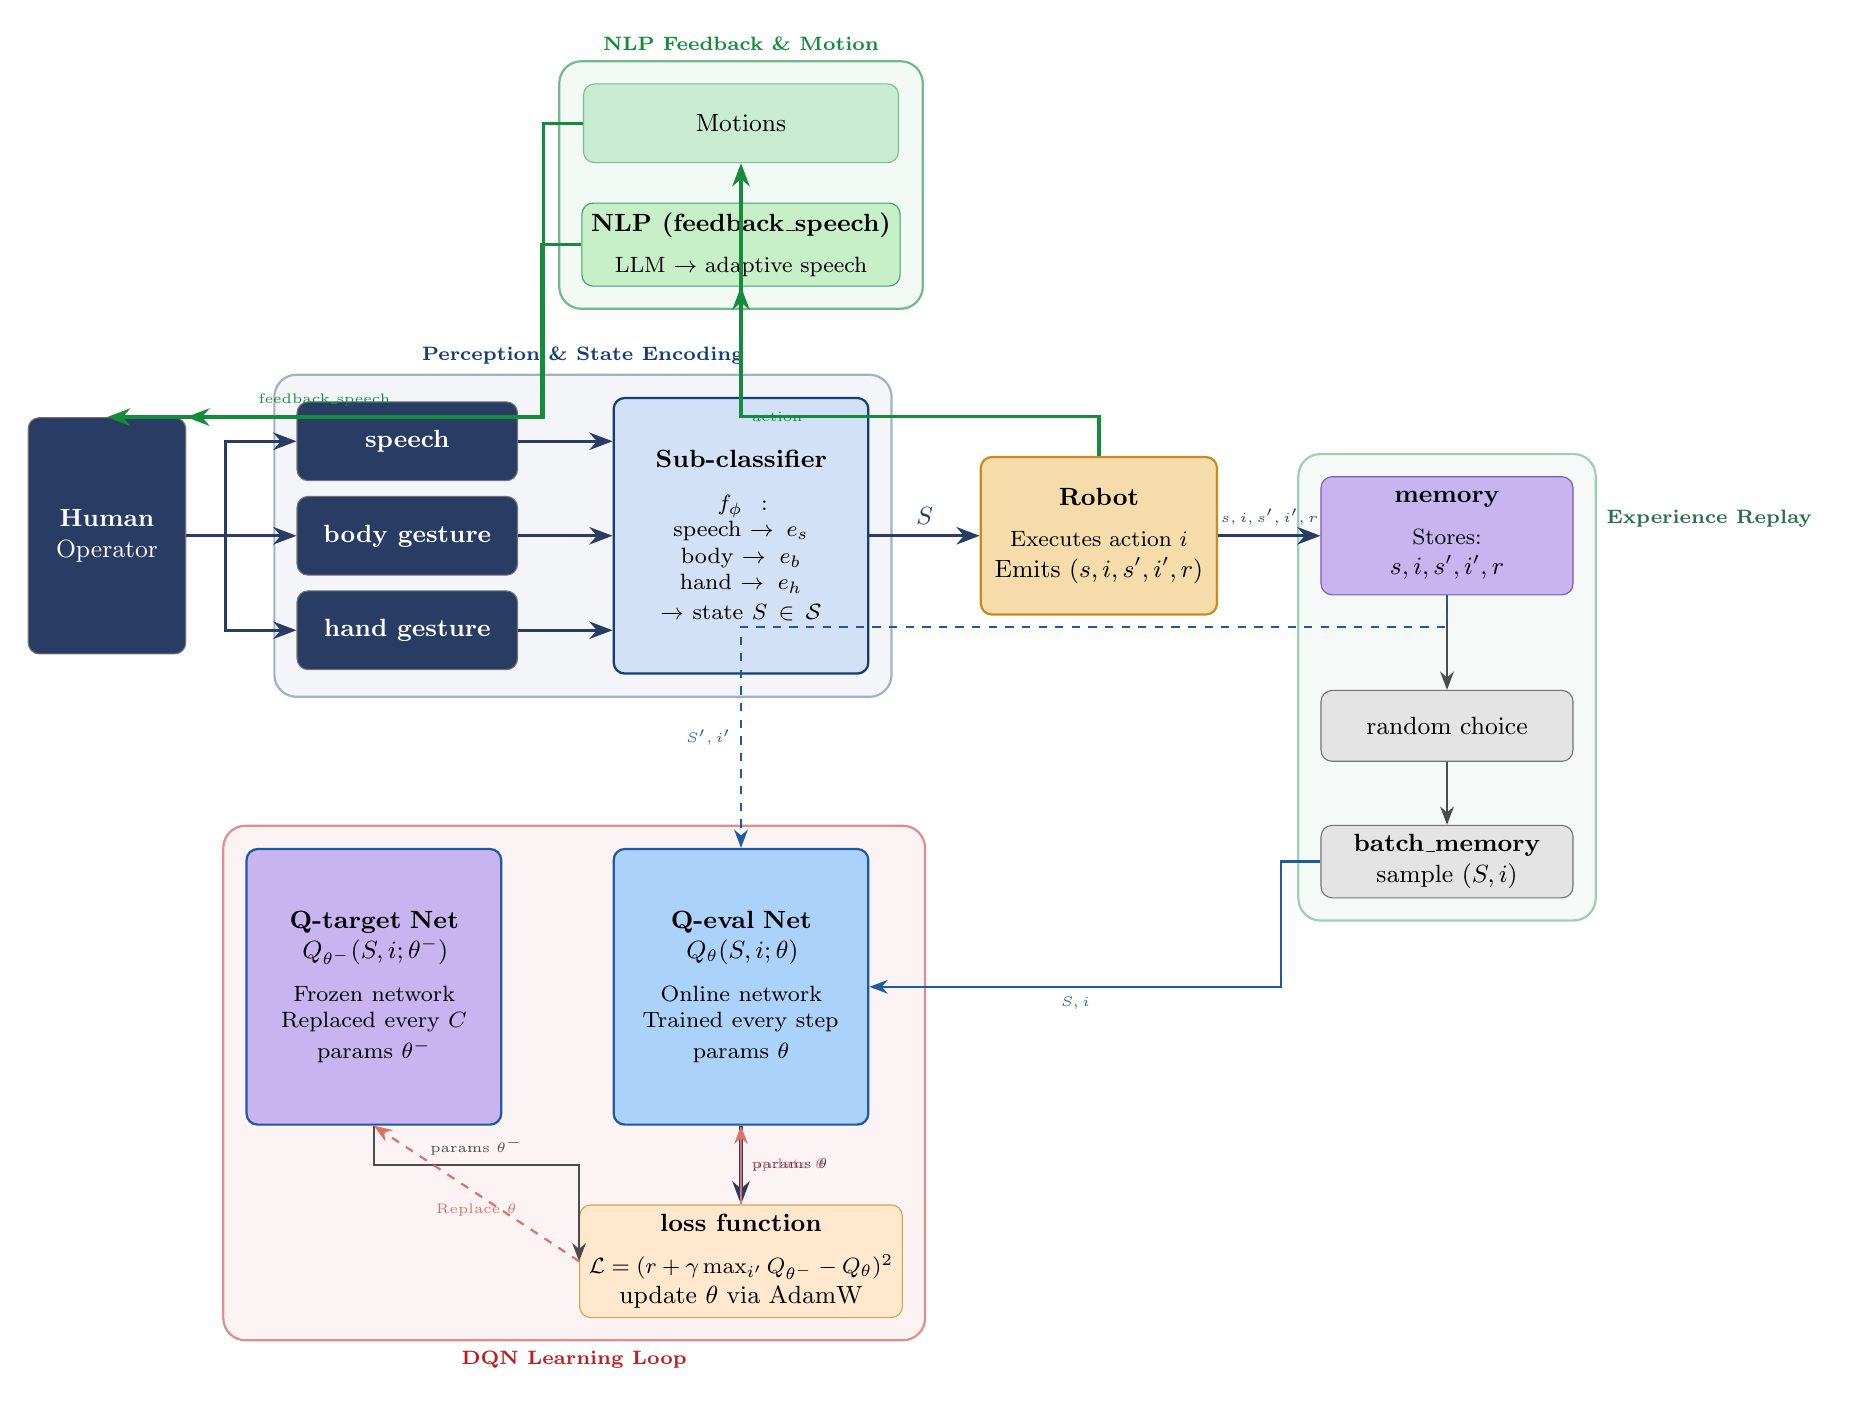
\begin{tikzpicture}[node distance=0.9cm and 1.1cm]

  %% Human operator
  \node[basebox,fill=cDark,text=white,minimum width=2.0cm,minimum height=3.0cm] (human) at (0,0)
    {\textbf{Human}\\Operator};

  %% Input streams
  \node[inputnode,right=1.4cm of human,yshift=1.2cm,minimum width=2.8cm] (speech)
    {speech};
  \node[inputnode,right=1.4cm of human,minimum width=2.8cm] (body)
    {body gesture};
  \node[inputnode,right=1.4cm of human,yshift=-1.2cm,minimum width=2.8cm] (hand)
    {hand gesture};

  %% Sub-classifier
  \node[subclnode,right=1.2cm of body,minimum width=3.2cm,minimum height=3.5cm,
        text width=3.0cm] (subclf)
    {\textbf{Sub-classifier}\\[6pt]
     \footnotesize$f_\phi:$\\
     speech $\to e_s$\\
     body $\to e_b$\\
     hand $\to e_h$\\
     $\to$ state $S \in \mathcal{S}$};

  %% Robot
  \node[robotnode,right=1.4cm of subclf,minimum width=3.0cm,minimum height=2.0cm] (robot)
    {\textbf{Robot}\\[4pt]\footnotesize Executes action $i$\\
     Emits $(s,i,s',i',r)$};

  %% Memory
  \node[memnode,right=1.3cm of robot,minimum width=3.2cm,minimum height=1.5cm] (memory)
    {\textbf{memory}\\[4pt]\footnotesize Stores:\\$s,i,s',i',r$};

  %% Random choice / batch_memory
  \node[datanode,below=1.2cm of memory,minimum width=3.2cm] (rand)
    {random choice};
  \node[datanode,below=0.8cm of rand,minimum width=3.2cm] (bmem)
    {\textbf{batch\_memory}\\sample $(S, i)$};

  %% Q-eval Net
  \node[qnetnode,below=2.2cm of subclf,minimum width=3.2cm,minimum height=3.5cm,
        text width=3.0cm] (qeval)
    {\textbf{Q-eval Net}\\$\Qeval(S,i;\theta)$\\[6pt]
     \footnotesize Online network\\
     Trained every step\\
     params $\theta$};

  %% Q-target Net
  \node[qnetnode,left=1.4cm of qeval,minimum width=3.2cm,minimum height=3.5cm,
        text width=3.0cm,fill=memorycol] (qtgt)
    {\textbf{Q-target Net}\\$\Qtgt(S,i;\theta^-)$\\[6pt]
     \footnotesize Frozen network\\
     Replaced every $C$\\
     params $\theta^-$};

  %% Loss function
  \node[lossnode,below=1.0cm of qeval,minimum width=3.6cm,minimum height=1.4cm] (loss)
    {\textbf{loss function}\\[4pt]
     \footnotesize $\Loss = (r+\gamma\max_{i'}\Qtgt - \Qeval)^2$\\
     update $\theta$ via AdamW};

  %% NLP node
  \node[nlpnode,above=1.4cm of subclf,minimum width=4.0cm] (nlp)
    {\textbf{NLP (feedback\_speech)}\\[4pt]
     \footnotesize LLM $\to$ adaptive speech};

  %% Motions node
  \node[retnode,above=0.5cm of nlp,minimum width=4.0cm] (motions)
    {Motions};

  %% ── ARROWS ──────────────────────────────────────────────
  %% Human → inputs
  \draw[thickarr] (human.east) -- ++(0.5,0) |- (speech.west);
  \draw[thickarr] (human.east) -- ++(0.5,0) |- (body.west);
  \draw[thickarr] (human.east) -- ++(0.5,0) |- (hand.west);

  %% inputs → sub-classifier
  \draw[thickarr] (speech.east) -- (subclf.west|-speech);
  \draw[thickarr] (body.east) -- (subclf.west|-body);
  \draw[thickarr] (hand.east) -- (subclf.west|-hand);

  %% sub-classifier → robot
  \draw[thickarr] (subclf.east) -- node[above,font=\small\bfseries]{$S$} (robot.west);

  %% robot → memory
  \draw[thickarr] (robot.east) -- node[above,font=\tiny]{$s,i,s',i',r$} (memory.west);

  %% memory → rand → batch_memory
  \draw[arr] (memory.south) -- (rand.north);
  \draw[arr] (rand.south) -- (bmem.north);

  %% batch_memory → Q-eval (S,i labels)
  \draw[bluearr] (bmem.west) -- ++(-0.5,0) |- node[near end,below,font=\tiny]{$S,i$} (qeval.east);

  %% Q-eval → loss
  \draw[thickarr] (qeval.south) -- node[right,font=\tiny]{params $\theta$} (loss.north);

  %% Q-target → loss (Replace θ)
  \draw[arr] (qtgt.south) -- ++(0,-0.5) -| (loss.west)
      node[near start,above,font=\tiny]{params $\theta^-$};

  %% loss → update θ on Q-eval
  \draw[redarr] (loss.north) -- node[right,font=\tiny]{update $\theta$} (qeval.south);

  %% loss → replace θ on Q-target
  \draw[redarr,dashed] (loss.west) -- (qtgt.south)
      node[midway,below,font=\tiny]{Replace $\theta$};

  %% memory → Q-eval: S',i'
  \draw[bluearr,dashed] (memory.south) -- ++(0,-0.4) -| (qeval.north)
      node[near end,left,font=\tiny]{$S',i'$};

  %% NLP ← robot (feedback)
  \draw[feedarr] (robot.north) -- ++(0,0.5) -| (nlp.south)
      node[midway,right,font=\tiny]{action};
  \draw[feedarr] (nlp.west) -- ++(-0.5,0) |- (human.north)
      node[near end,above,font=\tiny]{feedback\_speech};

  %% Motions ← robot
  \draw[feedarr] (robot.north) -- ++(0,0.5) -| (motions.south);
  \draw[feedarr] (motions.west) -- ++(-0.5,0) |- (human.north east);

  %% Background containers
  \begin{pgfonlayer}{background}
    \node[rectangle,draw=navyblue!40,fill=navyblue!5,rounded corners=8pt,thick,
          fit=(speech)(body)(hand)(subclf),inner sep=8pt,
          label={[font=\scriptsize\bfseries,color=navyblue]above:Perception \& State Encoding}] {};
    \node[rectangle,draw=mintgreen!50,fill=mintgreen!5,rounded corners=8pt,thick,
          fit=(memory)(rand)(bmem),inner sep=8pt,
          label={[font=\scriptsize\bfseries,color=mintgreen!70!black]above right:Experience Replay}] {};
    \node[rectangle,draw=lossred!50,fill=lossred!5,rounded corners=8pt,thick,
          fit=(qeval)(qtgt)(loss),inner sep=8pt,
          label={[font=\scriptsize\bfseries,color=lossred]below:DQN Learning Loop}] {};
    \node[rectangle,draw=rlgreen!60,fill=rlgreen!5,rounded corners=8pt,thick,
          fit=(nlp)(motions),inner sep=8pt,
          label={[font=\scriptsize\bfseries,color=rlgreen]above:NLP Feedback \& Motion}] {};
  \end{pgfonlayer}

\end{tikzpicture}
}
\caption{Complete MIVA-KNIGHT-RL closed-loop architecture. Human multimodal inputs (speech, body, hand gesture) are encoded by a sub-classifier into state $S$. A robot executes action $i$ and logs transitions $(s,i,s',i',r)$ to memory. Experience replay supplies training batches to Q-eval; the loss function trains $\theta$ and periodically replaces $\theta^-$ in Q-target. An NLP module generates adaptive speech feedback; a motion translator drives the robot's physical motions.}
\label{fig:full_rl_loop}
\end{figure}

%%
%% ============================================================
%% PART IV — MULTIMODAL INPUT AND SUB-CLASSIFIER
%% ============================================================
%%
\newpage
\section{Multimodal Input Processing and Sub-Classifier}
\label{sec:inputs}

\subsection{Three-Channel Human Input}
\label{sec:inputs_channels}

The system receives three concurrent input streams from the human operator:

\begin{definition}[Speech Input]
A spoken utterance $x_s \in \R^{T_s}$ (raw 16\,kHz waveform). Processed by Whisper (for transcript $q$) and Wav2Vec~2.0 (for emotion-aware embedding $e_s \in \R^{768}$).
\end{definition}

\begin{definition}[Body Gesture Input]
A sequence of joint-angle vectors or skeleton keypoints $x_b \in \R^{T_b \times J}$ where $J$ is the number of skeleton joints. Encoded by a temporal convolutional network or BERT-variant operating on the keypoint sequence.
\end{definition}

\begin{definition}[Hand Gesture Input]
A cropped hand-region image sequence $x_h \in \R^{T_h \times 3 \times H \times W}$. Encoded by ResNet-50 per frame followed by mean-temporal pooling to $e_h \in \R^{2048}$ then projected to $\R^{512}$.
\end{definition}

\subsection{Sub-Classifier Architecture}
\label{sec:subclassifier}

\begin{definition}[Sub-Classifier $f_\phi$]
The sub-classifier maps the three modality embeddings to a discrete state $S \in \mathcal{S}$:
\[
  f_\phi : \R^{d_s} \times \R^{d_b} \times \R^{d_h} \to \mathcal{S}, \quad |\mathcal{S}| = N_S
\]
where $d_s = 512$ (speech), $d_b = 512$ (body), $d_h = 512$ (hand). The fusion proceeds via:
\[
  e_{\text{fused}} = \phi(e_s, e_b, e_h) = \LN\!\left(W_f [e_s; e_b; e_h] + b_f\right) \in \R^{512}
\]
\[
  S = \argmax_{j \in \{1,\ldots,N_S\}} W_c e_{\text{fused}} + b_c
\]
\end{definition}

\begin{figure}[H]
\centering
\begin{adjustbox}{max width=\textwidth}
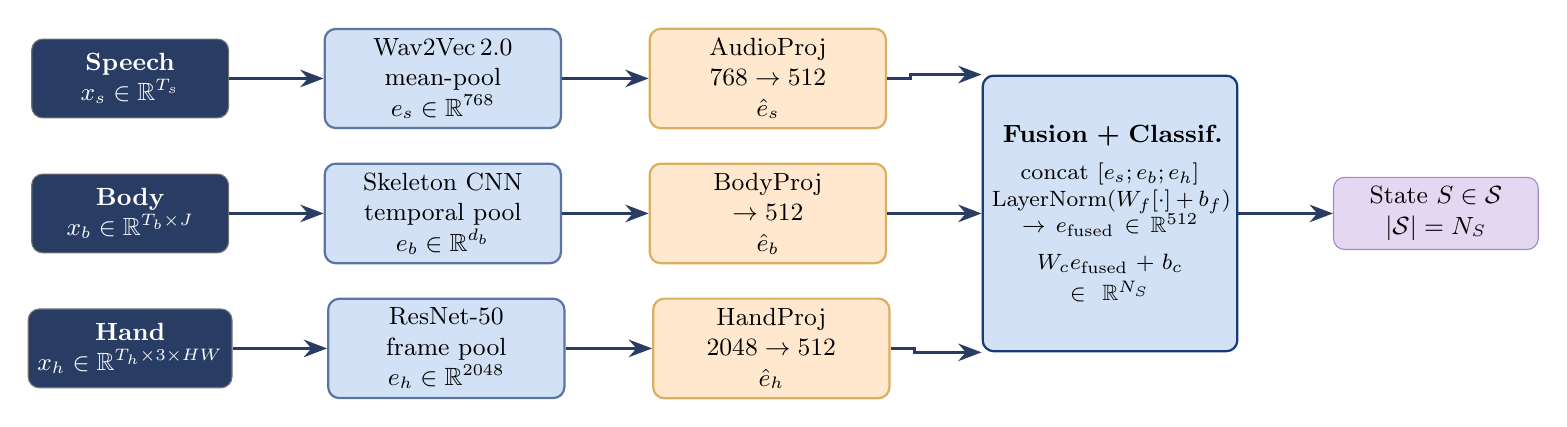
\begin{tikzpicture}[node distance=0.6cm and 0.8cm]
  \node[inputnode,minimum width=2.5cm] (sph) {Speech\\$x_s \in \R^{T_s}$};
  \node[inputnode,minimum width=2.5cm,below=0.7cm of sph] (bod) {Body\\$x_b \in \R^{T_b\times J}$};
  \node[inputnode,minimum width=2.5cm,below=0.7cm of bod] (hnd) {Hand\\$x_h \in \R^{T_h\times3\times HW}$};

  \node[encnode,right=1.2cm of sph,minimum width=3.0cm] (es)
    {Wav2Vec\,2.0\\mean-pool\\$e_s \in \R^{768}$};
  \node[encnode,right=1.2cm of bod,minimum width=3.0cm] (eb)
    {Skeleton CNN\\temporal pool\\$e_b \in \R^{d_b}$};
  \node[encnode,right=1.2cm of hnd,minimum width=3.0cm] (eh)
    {ResNet-50\\frame pool\\$e_h \in \R^{2048}$};

  \node[projnode,right=1.1cm of es] (ps) {AudioProj\\$768\to512$\\$\hat{e}_s$};
  \node[projnode,right=1.1cm of eb] (pb) {BodyProj\\$\to512$\\$\hat{e}_b$};
  \node[projnode,right=1.1cm of eh] (ph) {HandProj\\$2048\to512$\\$\hat{e}_h$};

  \node[subclnode,right=1.2cm of pb,minimum width=3.2cm,minimum height=3.5cm,
        yshift=0cm,text width=3.0cm] (fuse)
    {\textbf{Fusion + Classif.}\\[4pt]
     \footnotesize concat $[e_s;e_b;e_h]$\\
     $\LN(W_f[\cdot]+b_f)$\\
     $\to e_\text{fused}\in\R^{512}$\\[4pt]
     $W_c e_\text{fused}+b_c$\\
     $\in\R^{N_S}$};

  \node[outnode,right=1.2cm of fuse,minimum width=2.6cm] (state)
    {State $S \in \mathcal{S}$\\$|\mathcal{S}|=N_S$};

  \draw[thickarr] (sph)--(es); \draw[thickarr] (bod)--(eb); \draw[thickarr] (hnd)--(eh);
  \draw[thickarr] (es)--(ps); \draw[thickarr] (eb)--(pb); \draw[thickarr] (eh)--(ph);
  \draw[thickarr] (ps.east) -- ++(0.3,0) |- (fuse.north west);
  \draw[thickarr] (pb.east) -- (fuse.west);
  \draw[thickarr] (ph.east) -- ++(0.3,0) |- (fuse.south west);
  \draw[thickarr] (fuse)--(state);
\end{tikzpicture}
\end{adjustbox}
\caption{Sub-classifier architecture: three modality encoders produce 512-d embeddings; fusion layer concatenates and classifies to discrete state $S$.}
\label{fig:subclassifier}
\end{figure}

\begin{algorithm}[H]
\caption{Sub-Classifier Forward Pass: Multimodal State Encoding}
\label{alg:subclassifier}
\begin{algorithmic}[1]
\Require speech waveform $x_s$; body keypoints $x_b$; hand frames $x_h$
\Require Wav2Vec encoder $f_s$; body CNN $f_b$; ResNet-50 $f_h$
\Require Projection heads $P_s, P_b, P_h$ (each $\to \R^{512}$)
\Require Fusion layer $W_f, b_f \in \R^{512 \times 1536}$; classifier $W_c, b_c \in \R^{N_S}$
\Ensure Discrete state $S \in \{1,\ldots,N_S\}$, fused embedding $e_{\text{fused}}$
\State \textbf{// Stream A: Speech}
\State $h_s \gets f_s(x_s).\text{mean\_pool}()$ \Comment{Wav2Vec 2.0, $[768]$}
\State $\hat{e}_s \gets P_s(h_s) / \Norm{P_s(h_s)}_2$ \Comment{Project \& L2-norm, $[512]$}
\State \textbf{// Stream B: Body Gesture}
\State $h_b \gets f_b(x_b).\text{temporal\_pool}()$ \Comment{Skeleton CNN, $[d_b]$}
\State $\hat{e}_b \gets P_b(h_b) / \Norm{P_b(h_b)}_2$ \Comment{$[512]$}
\State \textbf{// Stream C: Hand Gesture}
\State $h_h \gets f_h(x_h).\text{global\_avg\_pool}()$ \Comment{ResNet-50 GAP, $[2048]$}
\State $\hat{e}_h \gets P_h(h_h) / \Norm{P_h(h_h)}_2$ \Comment{$[512]$}
\State \textbf{// Fusion}
\State $c \gets [\hat{e}_s;\, \hat{e}_b;\, \hat{e}_h] \in \R^{1536}$ \Comment{Concatenate}
\State $e_{\text{fused}} \gets \LN(W_f c + b_f) \in \R^{512}$
\State \textbf{// Classification to discrete state}
\State $\text{logits} \gets W_c e_{\text{fused}} + b_c \in \R^{N_S}$
\State $S \gets \argmax(\text{logits})$
\State \Return $(S,\; e_{\text{fused}})$
\end{algorithmic}
\end{algorithm}

\begin{tcolorbox}[laymanbox]
The sub-classifier is the robot's ``perception module''. It simultaneously reads what the operator says (speech), how they move their body (body gesture), and what their hands are doing (hand gesture). It combines all three signals into a single compact description — the state $S$ — which the DQN agent uses to decide what action the robot should take next.
\end{tcolorbox}

\begin{axiom}[State Completeness]
For the Markov property to hold, the state $S = f_\phi(x_s, x_b, x_h)$ must encode all information from the three input channels relevant to the robot's future. Any modality that is ignored introduces partial observability, converting the MDP into a POMDP.
\end{axiom}

\begin{definition}[Sub-Classifier Training Objective]
Given labelled dataset $\{(x_s^{(n)}, x_b^{(n)}, x_h^{(n)}, y_n)\}$ where $y_n \in \mathcal{S}$:
\[
  \Loss_{\text{clf}} = -\frac{1}{N}\sum_{n=1}^N \log P(S = y_n \mid x_s^{(n)}, x_b^{(n)}, x_h^{(n)};\; \phi)
\]
\[
  P(S = j \mid \cdot) = \softmax(W_c e_{\text{fused}})_j
\]
\end{definition}

\begin{algorithm}[H]
\caption{Sub-Classifier Training Loop}
\label{alg:subclf_train}
\begin{algorithmic}[1]
\Require Labelled dataset $\mathcal{D}$; batch size $B$; optimizer AdamW($\phi$, lr=$10^{-4}$)
\Ensure Trained sub-classifier parameters $\phi^*$
\For{epoch $= 1$ to $E_{\text{clf}}$}
  \ForEach{batch $\{(x_s, x_b, x_h, y)\}_{i=1}^B$ in $\mathcal{D}$}
    \State $(S_{\text{pred}}, e_f) \gets f_\phi(x_s, x_b, x_h)$ \Comment{Alg.~\ref{alg:subclassifier}}
    \State $\Loss \gets \text{CrossEntropy}(\text{logits}, y)$
    \State optimizer.zero\_grad(); $\Loss$.backward()
    \State clip\_grad\_norm$(\phi, c=1.0)$; optimizer.step()
  \EndFor
\EndFor
\State \Return $\phi^*$
\end{algorithmic}
\end{algorithm}

%%
%% ============================================================
%% PART V — ROBOT ACTION SPACE AND TRANSITION GENERATION
%% ============================================================
%%
\newpage
\section{Robot: Action Space and Transition Generation}
\label{sec:robot}

\subsection{Action Space and Policy}

\begin{definition}[Robot Action Space $\mathcal{A}$]
The robot's discrete action space is $\mathcal{A} = \{a_1, a_2, \ldots, a_m\}$ where each $a_j$ is a primitive robot motion (e.g., move-forward, turn-left, pick-up, wave, stop). The DQN $\varepsilon$-greedy policy selects:
\[
  i_t = \begin{cases}
    \text{random } a \sim \mathcal{A} & \text{with probability } \varepsilon \\
    \argmax_{a} \Qeval(S_t, a;\; \theta) & \text{with probability } 1 - \varepsilon
  \end{cases}
\]
\end{definition}

\begin{definition}[Typed Transition Tuple]
The MIVA-KNIGHT-RL system stores \textbf{typed transitions} with two action indices:
\[
  \tau = (s,\; i,\; s',\; i',\; r)
\]
where:
\begin{itemize}[nosep]
  \item $s$: current state (encoded by sub-classifier)
  \item $i$: action taken at $s$ (modality-action pair index)
  \item $s'$: next state after executing $i$
  \item $i'$: action selected at $s'$ (greedy under current $\theta$; used for SARSA-style updates)
  \item $r$: reward received
\end{itemize}
\end{definition}

\begin{remark}[DQN vs. SARSA Transitions]
Standard DQN stores $(s, a, r, s')$ and uses $\max_{a'} Q(s', a')$ for the target. The MIVA-KNIGHT-RL formulation stores $(s, i, s', i', r)$, where $i'$ is logged for potential SARSA-style ($Q(s', i')$) or double-DQN variants.
\end{remark}

\begin{figure}[H]
\centering
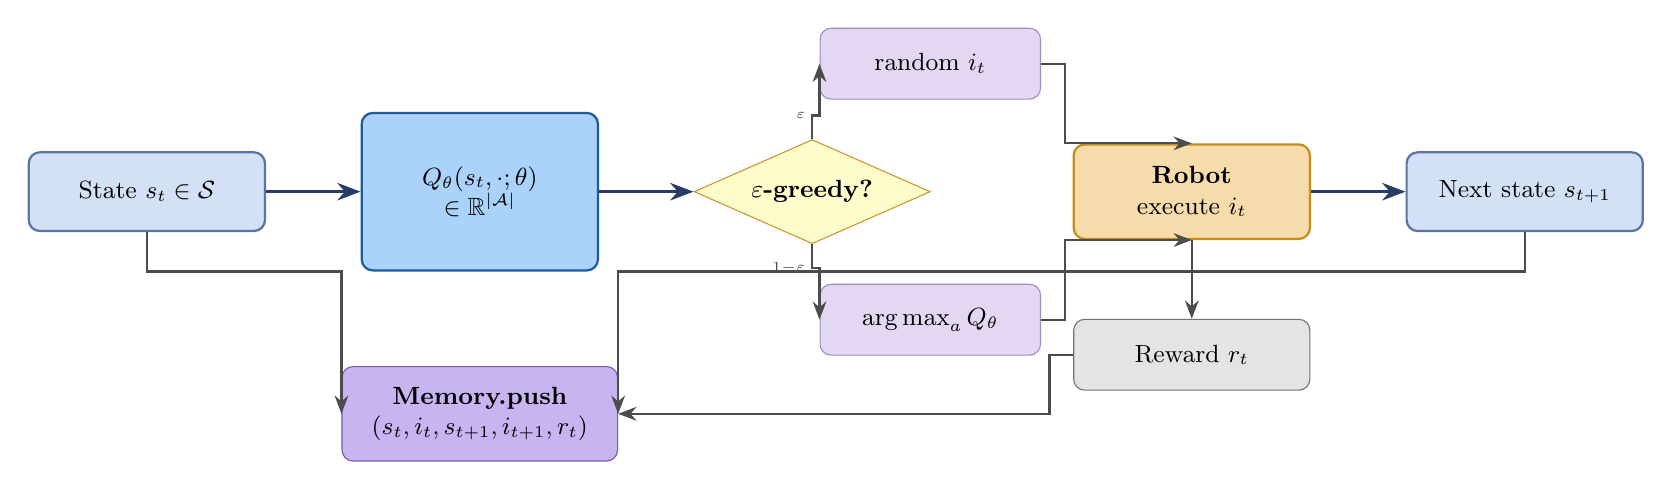
\begin{tikzpicture}[node distance=0.7cm and 1.2cm]
  \node[encnode,minimum width=3.0cm] (st) {State $s_t \in \mathcal{S}$};
  \node[qnetnode,right=1.2cm of st,minimum width=3.0cm,minimum height=2.0cm] (qev)
    {$\Qeval(s_t, \cdot;\theta)$\\$\in\R^{|\mathcal{A}|}$};
  \node[decnode,right=1.2cm of qev] (eps) {$\varepsilon$-greedy?};
  \node[outnode,above=0.5cm of eps,xshift=1.5cm] (rand2) {random $i_t$};
  \node[outnode,below=0.5cm of eps,xshift=1.5cm] (greedy) {$\argmax_a \Qeval$};
  \node[robotnode,right=1.8cm of eps,minimum width=3.0cm] (rob)
    {\textbf{Robot}\\execute $i_t$};
  \node[encnode,right=1.2cm of rob,minimum width=3.0cm] (sp) {Next state $s_{t+1}$};
  \node[datanode,below=1.0cm of rob,minimum width=3.0cm] (rew) {Reward $r_t$};
  \node[memnode,below=1.2cm of qev,minimum width=3.5cm] (mem)
    {\textbf{Memory.push}\\$(s_t, i_t, s_{t+1}, i_{t+1}, r_t)$};

  \draw[thickarr] (st)--(qev);
  \draw[thickarr] (qev)--(eps);
  \draw[arr] (eps.north) -- ++(0,0.3) -| (rand2.west) node[near start,left,font=\tiny]{$\varepsilon$};
  \draw[arr] (eps.south) -- ++(0,-0.3) -| (greedy.west) node[near start,left,font=\tiny]{$1{-}\varepsilon$};
  \draw[arr] (rand2.east) -- ++(0.3,0) |- (rob.north);
  \draw[arr] (greedy.east) -- ++(0.3,0) |- (rob.south);
  \draw[thickarr] (rob.east) -- (sp.west);
  \draw[arr] (rob.south) -- (rew.north);
  \draw[arr] (sp.south) -- ++(0,-0.5) -| (mem.east);
  \draw[arr] (rew.west) -- ++(-0.3,0) |- (mem.east);
  \draw[arr] (st.south) -- ++(0,-0.5) -| (mem.west);
\end{tikzpicture}
\caption{Robot transition generation: $\varepsilon$-greedy action selection, execution, and transition storage.}
\label{fig:transition_gen}
\end{figure}

\begin{algorithm}[H]
\caption{Robot Interaction and Transition Generation}
\label{alg:robot_interact}
\begin{algorithmic}[1]
\Require Current state $s_t$; Q-eval $\Qeval(\cdot;\theta)$; $\varepsilon$; memory buffer $\mathcal{B}$
\Ensure Next state $s_{t+1}$; stored transition $\tau$
\State \textbf{// $\varepsilon$-greedy action selection}
\If{uniform$(0,1) < \varepsilon$}
  \State $i_t \gets \text{uniform\_sample}(\mathcal{A})$ \Comment{Exploration}
\Else
  \State $i_t \gets \argmax_{a} \Qeval(s_t, a;\theta)$ \Comment{Exploitation}
\EndIf
\State \textbf{// Execute action on robot}
\State Execute robot primitive $a_{i_t}$ on physical/simulated robot
\State Observe: $s_{t+1} \gets f_\phi(x_s^{t+1}, x_b^{t+1}, x_h^{t+1})$ \Comment{Next state via sub-classifier}
\State $r_t \gets \mathcal{R}(s_t, i_t, s_{t+1})$ \Comment{Reward signal}
\State \textbf{// Compute next action (for $i'$ in SARSA-style logging)}
\State $i_{t+1} \gets \argmax_a \Qeval(s_{t+1}, a;\theta)$ \Comment{Greedy next action}
\State \textbf{// Store transition in replay memory}
\State $\mathcal{B}.\text{push}(\tau = (s_t, i_t, s_{t+1}, i_{t+1}, r_t))$
\State \textbf{// Decay exploration rate}
\State $\varepsilon \gets \max(\varepsilon_{\min}, \varepsilon \cdot \varepsilon_{\text{decay}})$
\State \Return $(s_{t+1}, \tau)$
\end{algorithmic}
\end{algorithm}

\begin{definition}[Reward Function]
\[
  r_t = \mathcal{R}(s_t, i_t, s_{t+1}) = w_1 r_{\text{task}} + w_2 r_{\text{safety}} + w_3 r_{\text{social}},
  \quad w_1 + w_2 + w_3 = 1
\]
where $r_{\text{task}}$ rewards goal completion, $r_{\text{safety}} \in \{-1, 0\}$ penalises unsafe actions, and $r_{\text{social}}$ rewards appropriate multimodal gesture alignment.
\end{definition}

%%
%% ============================================================
%% PART VI — EXPERIENCE REPLAY MEMORY
%% ============================================================
%%
\newpage
\section{Experience Replay Memory}
\label{sec:memory}

\subsection{Replay Buffer Design}

\begin{definition}[Replay Buffer]
The replay buffer $\mathcal{B}$ is a fixed-capacity ring buffer of transitions:
\[
  \mathcal{B} = \{(s^{(j)}, i^{(j)}, {s'}^{(j)}, {i'}^{(j)}, r^{(j)})\}_{j=1}^{|\mathcal{B}|}
\]
with capacity $|\mathcal{B}| = C_{\mathcal{B}}$. When full, the oldest transition is overwritten (FIFO).
\end{definition}

\begin{axiom}[Decorrelation via Replay]
Consecutive environment transitions $(s_t, i_t, s_{t+1}, r_t)$ are highly correlated. Training on correlated mini-batches causes oscillating Q-value updates. Uniform random sampling from $\mathcal{B}$ produces an approximately i.i.d.\ mini-batch, reducing update variance.
\end{axiom}

\begin{figure}[H]
\centering
\begin{adjustbox}{max width=\textwidth}
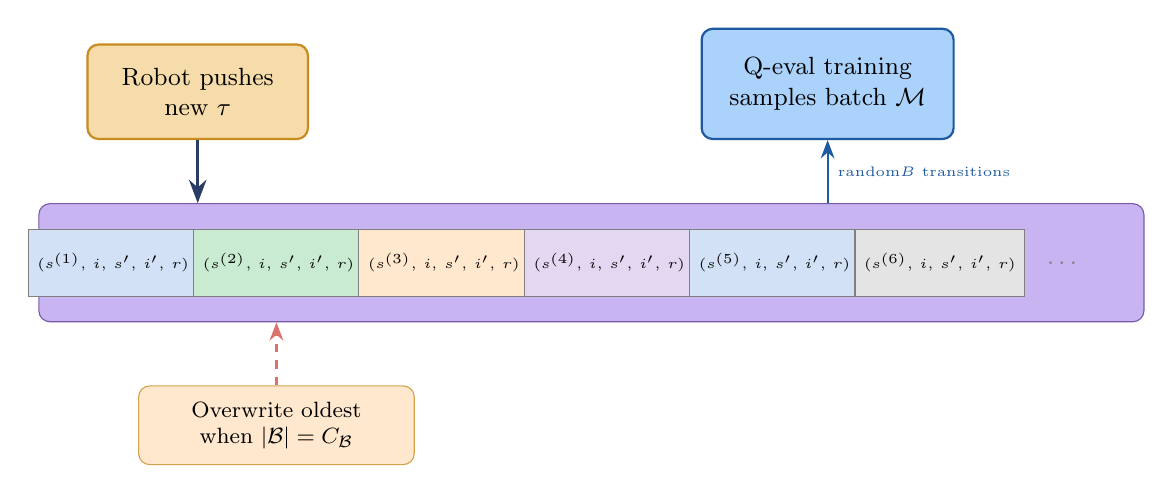
\begin{tikzpicture}[node distance=0.6cm and 1.0cm]
  %% Memory ring-buffer visualisation
  \node[memnode,minimum width=14cm,minimum height=1.5cm,text width=13.8cm] (buf)
    {\textbf{Replay Buffer $\mathcal{B}$} (ring buffer, capacity $C_\mathcal{B}$)};

  %% Individual transition slots
  \foreach \x/\clr in {0/boxblue,1/boxgreen,2/boxorange,3/boxpurple,4/boxblue,5/boxgray} {
    \node[rectangle,draw=black!50,fill=\clr,minimum width=1.9cm,minimum height=0.85cm,
          font=\tiny,align=center] at ($(buf.west)+(0.95+\x*2.1, -0.0)$)
      {$(s^{(\pgfmathparse{int(\x+1)}\pgfmathresult)},\,i,\,s',\,i',\,r)$};
  }
  \node[font=\small\bfseries,color=gray] at ($(buf.west)+(13.0,0)$) {$\ldots$};

  %% Push arrow
  \node[robotnode,above=0.8cm of buf,minimum width=2.8cm,xshift=-5cm] (push)
    {Robot pushes\\new $\tau$};
  \draw[thickarr] (push.south) -- (buf.north-|push);

  %% Sample arrow
  \node[qnetnode,above=0.8cm of buf,minimum width=3.2cm,minimum height=1.4cm,xshift=3cm] (sample)
    {Q-eval training\\samples batch $\mathcal{M}$};
  \draw[bluearr] (buf.north-|sample) -- node[right,font=\tiny]{random\\$B$ transitions} (sample.south);

  %% Overwrite indicator
  \node[lossnode,below=0.8cm of buf,minimum width=3.5cm,font=\footnotesize,xshift=-4cm] (ow)
    {Overwrite oldest\\when $|\mathcal{B}|=C_\mathcal{B}$};
  \draw[redarr,dashed] (ow.north) -- (buf.south-|ow);
\end{tikzpicture}
\end{adjustbox}
\caption{Replay buffer architecture: new transitions are pushed from the robot; training batches are sampled uniformly; the oldest transitions are overwritten when capacity is reached.}
\label{fig:replay_buffer}
\end{figure}

\begin{algorithm}[H]
\caption{Experience Replay Memory Operations}
\label{alg:replay_memory}
\begin{algorithmic}[1]
\Require Capacity $C_\mathcal{B}$; transition $\tau$; batch size $B$
\State \textbf{Initialise:} ring buffer $\mathcal{B}[0:C_\mathcal{B}-1]$; pointer $p \gets 0$; count $\gets 0$

\Procedure{Push}{$\tau = (s, i, s', i', r)$}
  \State $\mathcal{B}[p] \gets \tau$
  \State $p \gets (p + 1) \mod C_\mathcal{B}$ \Comment{Circular overwrite}
  \State count $\gets \min(\text{count} + 1, C_\mathcal{B})$
\EndProcedure

\Procedure{Sample}{$B$}
  \Require count $\ge B$ \Comment{At least $B$ transitions stored}
  \State $\mathcal{I} \gets \text{RandomChoice}(\{0,\ldots,\text{count}-1\}, B, \text{replace}=\text{False})$
  \State $\mathcal{M} \gets \{\mathcal{B}[j] : j \in \mathcal{I}\}$ \Comment{Uniformly sampled mini-batch}
  \State \Return $\mathcal{M}$
\EndProcedure

\Procedure{BatchMemory}{} \Comment{Structured batch for Q-network training}
  \State $\mathcal{M} \gets \Call{Sample}{B}$
  \State $S_{\text{batch}} \gets \text{stack}([s \text{ for } (s,i,s',i',r) \in \mathcal{M}])$
  \State $I_{\text{batch}} \gets \text{tensor}([i \text{ for } (s,i,s',i',r) \in \mathcal{M}])$
  \State $S'_{\text{batch}} \gets \text{stack}([s' \text{ for } (s,i,s',i',r) \in \mathcal{M}])$
  \State $I'_{\text{batch}} \gets \text{tensor}([i' \text{ for } (s,i,s',i',r) \in \mathcal{M}])$
  \State $R_{\text{batch}} \gets \text{tensor}([r \text{ for } (s,i,s',i',r) \in \mathcal{M}])$
  \State \Return $(S_{\text{batch}}, I_{\text{batch}}, S'_{\text{batch}}, I'_{\text{batch}}, R_{\text{batch}})$
\EndProcedure
\end{algorithmic}
\end{algorithm}

\begin{theorem}[Replay Buffer Minimum Size]
The replay buffer requires a warm-up phase of at least $|\mathcal{B}_{\text{min}}| = B$ transitions before training begins (where $B$ is the mini-batch size). Training before warm-up leads to biased sampling with replacement, inflating the effective gradient variance by a factor of $B / (|\mathcal{B}| - B + 1)$ for sampling without replacement.
\end{theorem}

\begin{tcolorbox}[rlbox]
Experience replay is the key insight that makes DQN stable. Without it, consecutive training samples are nearly identical (the robot's state changes slowly), causing the Q-network to ``over-fit'' to recent experience and forget earlier transitions. By storing and randomly re-mixing thousands of past interactions, replay ensures every gradient update sees a diverse, statistically independent slice of the robot's history.
\end{tcolorbox}

%%
%% ============================================================
%% PART VII — Q-EVALUATION NETWORK
%% ============================================================
%%
\newpage
\section{Q-Evaluation Network}
\label{sec:qeval}

\subsection{Architecture}

\begin{definition}[Q-Eval Network $\Qeval$]
The Q-eval network $\Qeval(s, a; \theta) : \mathcal{S} \times \mathcal{A} \to \R$ is implemented as a multi-layer perceptron that takes the state embedding $e_s \in \R^{d_s}$ as input and outputs $Q$-values for all actions simultaneously:
\[
  \Qeval(\cdot;\theta) : \R^{d_s} \to \R^{|\mathcal{A}|}, \quad
  \hat{q}_j = \Qeval(s, a_j; \theta)
\]
Architecture: $d_s \to 512 \to 256 \to |\mathcal{A}|$ with ReLU activations and LayerNorm after each hidden layer.
\end{definition}

\begin{figure}[H]
\centering
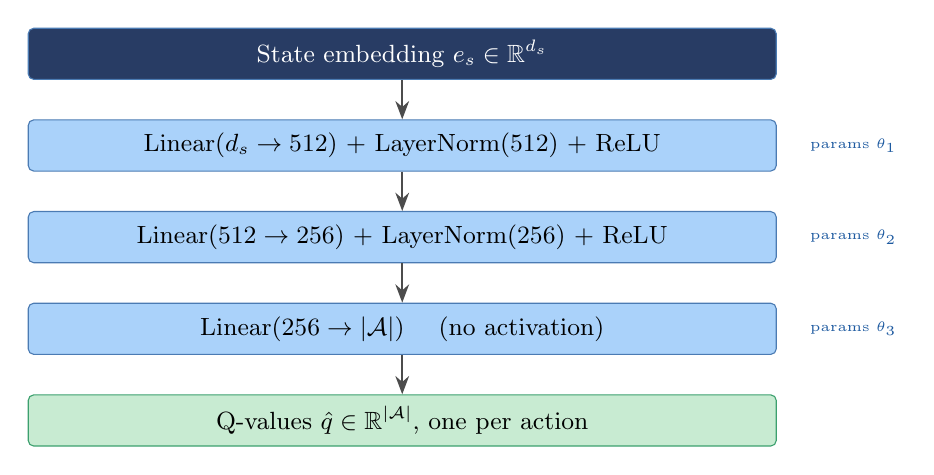
\begin{tikzpicture}[node distance=0.5cm and 0.9cm,
  layerstyle/.style={rectangle,rounded corners=2pt,draw=robotblue!80,fill=qnetcol,
    align=center,font=\small,minimum width=9.5cm,minimum height=0.65cm}]
  \node[layerstyle,fill=cDark,text=white] (inp) {State embedding $e_s \in \R^{d_s}$};
  \node[layerstyle,below=of inp] (l1) {Linear$(d_s \to 512)$ + LayerNorm(512) + ReLU};
  \node[layerstyle,below=of l1] (l2) {Linear$(512 \to 256)$ + LayerNorm(256) + ReLU};
  \node[layerstyle,below=of l2] (l3) {Linear$(256 \to |\mathcal{A}|)$ \quad (no activation)};
  \node[layerstyle,below=of l3,fill=boxgreen,draw=mintgreen] (out) {Q-values $\hat{q} \in \R^{|\mathcal{A}|}$, one per action};
  \foreach \a/\b in {inp/l1,l1/l2,l2/l3,l3/out} \draw[arr] (\a)--(\b);
  \node[right=0.3cm of l1,font=\tiny,color=robotblue] {params $\theta_1$};
  \node[right=0.3cm of l2,font=\tiny,color=robotblue] {params $\theta_2$};
  \node[right=0.3cm of l3,font=\tiny,color=robotblue] {params $\theta_3$};
\end{tikzpicture}
\caption{Q-eval network architecture. State embedding input; 3-layer MLP; Q-value output for all actions.}
\label{fig:qeval_arch}
\end{figure}

\subsection{Online Update Rule}

\begin{definition}[Q-Eval Update]
At each training step $t$, given mini-batch $\mathcal{M} = \{(s^{(j)}, i^{(j)}, {s'}^{(j)}, {i'}^{(j)}, r^{(j)})\}_{j=1}^B$:

\textbf{Step 1 — Compute TD targets using frozen $\theta^-$:}
\[
  y^{(j)} = r^{(j)} + \gamma \max_{a'} \Qtgt(s'^{(j)}, a';\; \theta^-)
\]

\textbf{Step 2 — Compute current Q-values:}
\[
  \hat{q}^{(j)} = \Qeval(s^{(j)}, i^{(j)};\; \theta)
\]

\textbf{Step 3 — TD loss (Huber):}
\[
  \Loss(\theta) = \frac{1}{B}\sum_{j=1}^B L_\delta\!\left(y^{(j)} - \hat{q}^{(j)}\right)
\]

\textbf{Step 4 — Gradient descent:}
\[
  \theta \gets \theta - \eta \nabla_\theta \Loss(\theta)
\]
\end{definition}

\begin{algorithm}[H]
\caption{Q-Eval Network Training Step}
\label{alg:qeval_step}
\begin{algorithmic}[1]
\Require Mini-batch $\mathcal{M}$ (from Alg.~\ref{alg:replay_memory}); $\Qeval(\cdot;\theta)$; $\Qtgt(\cdot;\theta^-)$; $\gamma$; optimizer
\Ensure Updated $\theta$; TD loss value
\State $(S, I, S', I', R) \gets \textsc{BatchMemory}(\mathcal{M})$ \Comment{Alg.~\ref{alg:replay_memory}}
\State \textbf{// Step 1: TD targets (frozen target network, no gradient)}
\State \textbf{with} torch.no\_grad():
\State $\quad Q'_{\text{max}} \gets \max_{a'} \Qtgt(S', a';\theta^-) \in \R^B$
  \Comment{Row-wise max over all actions}
\State $\quad Y \gets R + \gamma \cdot Q'_{\text{max}} \in \R^B$
  \Comment{Bootstrap target}
\State \textbf{// Step 2: Predicted Q-values for taken actions}
\State $Q_{\text{all}} \gets \Qeval(S;\theta) \in \R^{B \times |\mathcal{A}|}$
\State $\hat{Q} \gets Q_{\text{all}}[\text{range}(B),\; I] \in \R^B$
  \Comment{Select Q-value for each taken action $i^{(j)}$}
\State \textbf{// Step 3: Huber loss}
\State $\delta \gets Y - \hat{Q}$ \Comment{TD error $\in \R^B$}
\State $\Loss \gets \frac{1}{B}\sum_j L_\delta(\delta_j)$
  \Comment{Huber loss (smooth-L1)}
\State \textbf{// Step 4: Gradient update}
\State optimizer.zero\_grad(); $\Loss$.backward()
\State clip\_grad\_norm$(\theta, c=10.0)$
\State optimizer.step()
\State \Return $\Loss$.item()
\end{algorithmic}
\end{algorithm}

%%
%% ============================================================
%% PART VIII — Q-TARGET NETWORK AND REPLACEMENT
%% ============================================================
%%
\newpage
\section{Q-Target Network and Periodic Replacement}
\label{sec:qtarget}

\subsection{Why a Separate Target Network?}

\begin{definition}[Q-Target Network $\Qtgt$]
The Q-target network is an \textbf{exact copy} of the Q-eval network but with \textbf{frozen parameters} $\theta^-$. It is only updated every $C$ training steps by hard replacement:
\[
  \theta^- \gets \theta \quad \text{every } C \text{ steps}
\]
\end{definition}

\begin{theorem}[Non-Stationarity Without Target Network]
Without a target network, the loss is:
\[
  \Loss(\theta) = \EE\!\left[\left(r + \gamma\max_{a'}\Qeval(s',a';\theta) - \Qeval(s,a;\theta)\right)^2\right]
\]
Both target and prediction depend on $\theta$. The gradient
$\nabla_\theta \Loss = -2\delta_t \nabla_\theta \Qeval(s,a;\theta) - 2\delta_t \nabla_\theta (\gamma \max_{a'} \Qeval(s',a';\theta))$
includes a \emph{second term that pushes the target in the same direction as the prediction}, causing the target to ``chase'' the prediction and leading to oscillation or divergence.
\end{theorem}

\begin{proof}[Proof sketch]
Let $q = \Qeval(s,a;\theta)$ and $q' = \max_{a'}\Qeval(s',a';\theta)$ (same $\theta$). The loss is $(r + \gamma q' - q)^2$. Taking the gradient w.r.t.\ $\theta$:
\[
  \nabla_\theta \Loss = 2(r + \gamma q' - q)\left(-\nabla_\theta q + \gamma \nabla_\theta q'\right)
\]
The term $\gamma \nabla_\theta q'$ causes the target $r + \gamma q'$ to shift in the same direction as $q$ is being updated, creating a feedback loop. Setting $\nabla_\theta q' = 0$ (frozen target) eliminates this instability. \qed
\end{proof}

\begin{figure}[H]
\centering
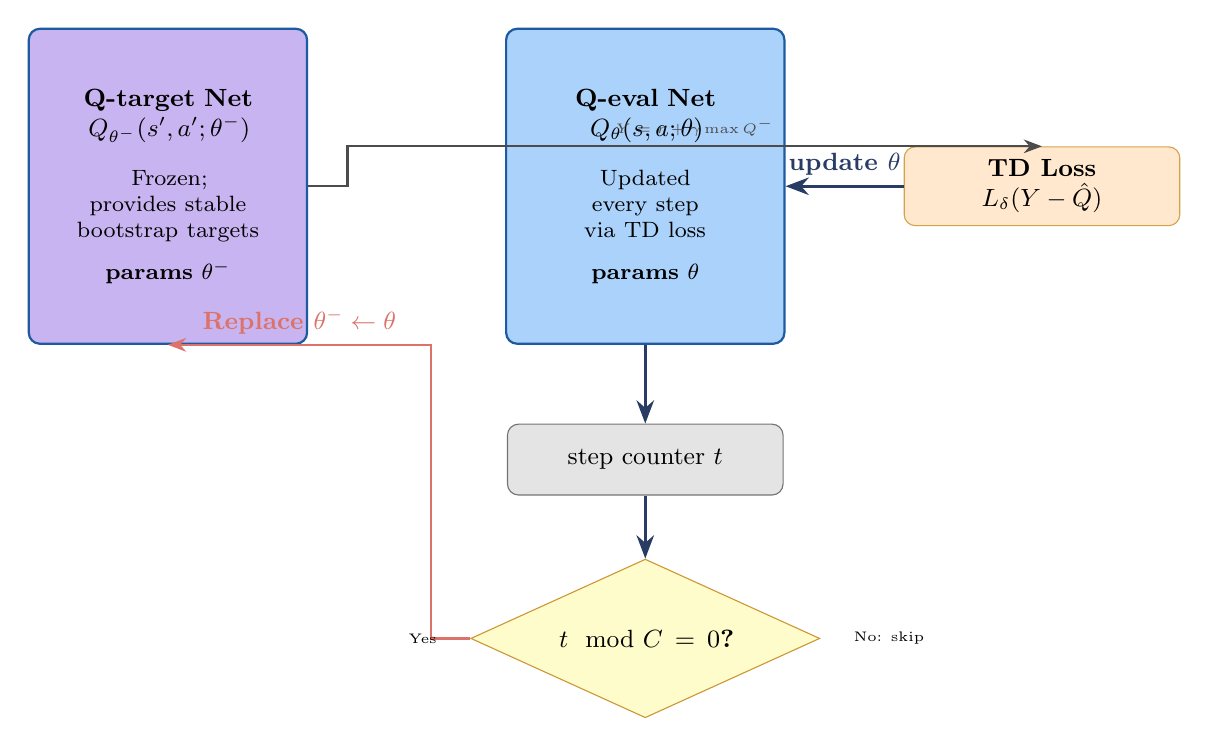
\begin{tikzpicture}[node distance=0.8cm and 1.3cm]
  %% Q-eval
  \node[qnetnode,minimum width=3.5cm,minimum height=4.0cm,text width=3.3cm] (qev2)
    {\textbf{Q-eval Net}\\$\Qeval(s,a;\theta)$\\[8pt]
     \footnotesize Updated\\every step\\via TD loss\\[4pt]
     \textbf{params $\theta$}};

  %% Q-target
  \node[qnetnode,fill=memorycol,minimum width=3.5cm,minimum height=4.0cm,
        text width=3.3cm,left=2.5cm of qev2] (qtgt2)
    {\textbf{Q-target Net}\\$\Qtgt(s',a';\theta^-)$\\[8pt]
     \footnotesize Frozen;\\provides stable\\bootstrap targets\\[4pt]
     \textbf{params $\theta^-$}};

  %% Counter
  \node[datanode,below=1.0cm of qev2,minimum width=3.5cm] (cnt)
    {step counter $t$};
  \node[decnode,below=0.8cm of cnt,minimum width=3.5cm,text width=3.2cm] (cmod)
    {$t \mod C = 0$?};

  %% Loss → Q-eval
  \node[lossnode,right=1.5cm of qev2,minimum width=3.5cm] (loss2)
    {\textbf{TD Loss}\\$L_\delta(Y - \hat{Q})$};

  %% Arrows
  \draw[thickarr] (loss2.west) -- node[above,font=\small\bfseries]{update $\theta$} (qev2.east);
  \draw[arr] (qtgt2.east) -- ++(0.5,0) |- node[near end,above,font=\tiny]{$Y = r+\gamma\max Q^-$} (loss2.north);
  \draw[thickarr] (qev2.south) -- (cnt.north);
  \draw[thickarr] (cnt.south) -- (cmod.north);
  \draw[redarr] (cmod.west) -- ++(-0.5,0) |- node[near end,above,font=\small\bfseries]{Replace $\theta^- \gets \theta$} (qtgt2.south);
  \node[font=\tiny,right=0.3cm of cmod] {No: skip};
  \node[font=\tiny,left=0.3cm of cmod] {Yes};
\end{tikzpicture}
\caption{Dual Q-network with periodic target replacement. Q-eval is updated every step; Q-target is replaced every $C$ steps.}
\label{fig:dual_qnet}
\end{figure}

\begin{algorithm}[H]
\caption{Target Network Management: Replace $\theta^-$}
\label{alg:target_replace}
\begin{algorithmic}[1]
\Require Q-eval $\Qeval(\cdot;\theta)$; Q-target $\Qtgt(\cdot;\theta^-)$;\\
         replacement interval $C$; current step counter $t$
\Ensure Updated $\theta^-$ (if replacement condition met)
\If{$t \mod C = 0$ \textbf{and} $t > 0$}
  \State $\theta^- \gets \theta$ \Comment{Hard copy all weights and biases}
  \State \textbf{Assert} $\Qtgt(s, a;\theta^-) = \Qeval(s, a;\theta)$ for test input $s$ \Comment{Sanity check}
  \State log ``Target network replaced at step $t$''
\EndIf
\State \Return $\theta^-$
\end{algorithmic}
\end{algorithm}

\begin{lemma}[Soft Target Update Alternative]
Instead of hard replacement, a \emph{soft update} (Polyak averaging) can be used:
\[
  \theta^- \gets \tau_{\text{soft}} \theta + (1 - \tau_{\text{soft}}) \theta^-, \quad \tau_{\text{soft}} \ll 1
\]
Soft updates trade stability for tracking speed. For $\tau_{\text{soft}} = 10^{-3}$, the target network changes at $\sim 0.1\%$ per step, preventing abrupt Q-value jumps.
\end{lemma}

%%
%% ============================================================
%% PART IX — LOSS FUNCTION AND OPTIMISATION
%% ============================================================
%%
\newpage
\section{Loss Function and Parameter Optimisation}
\label{sec:loss}

\subsection{TD-Error Loss}

\begin{definition}[Temporal Difference Error]
\[
  \delta_t = \underbrace{r_t + \gamma \max_{a'} \Qtgt(s_{t+1}, a';\theta^-)}_{\text{TD target } y_t} - \underbrace{\Qeval(s_t, a_t;\theta)}_{\text{current Q-value}}
\]
The TD error $\delta_t$ measures how much the current Q-estimate deviates from the bootstrapped estimate. Minimising $\EE[\delta_t^2]$ drives $\Qeval \to Q^*$.
\end{definition}

\begin{definition}[Full Training Objective]
\[
  \Loss(\theta) = \frac{1}{B}\sum_{j=1}^B L_\delta\!\left(r^{(j)} + \gamma \max_{a'} \Qtgt(s'^{(j)}, a';\theta^-) - \Qeval(s^{(j)}, i^{(j)};\theta)\right)
\]
where $L_\delta$ is the Huber loss with $\delta = 1$ (Lemma 2.2).
\end{definition}

\begin{figure}[H]
\centering
\begin{adjustbox}{max width=\textwidth}
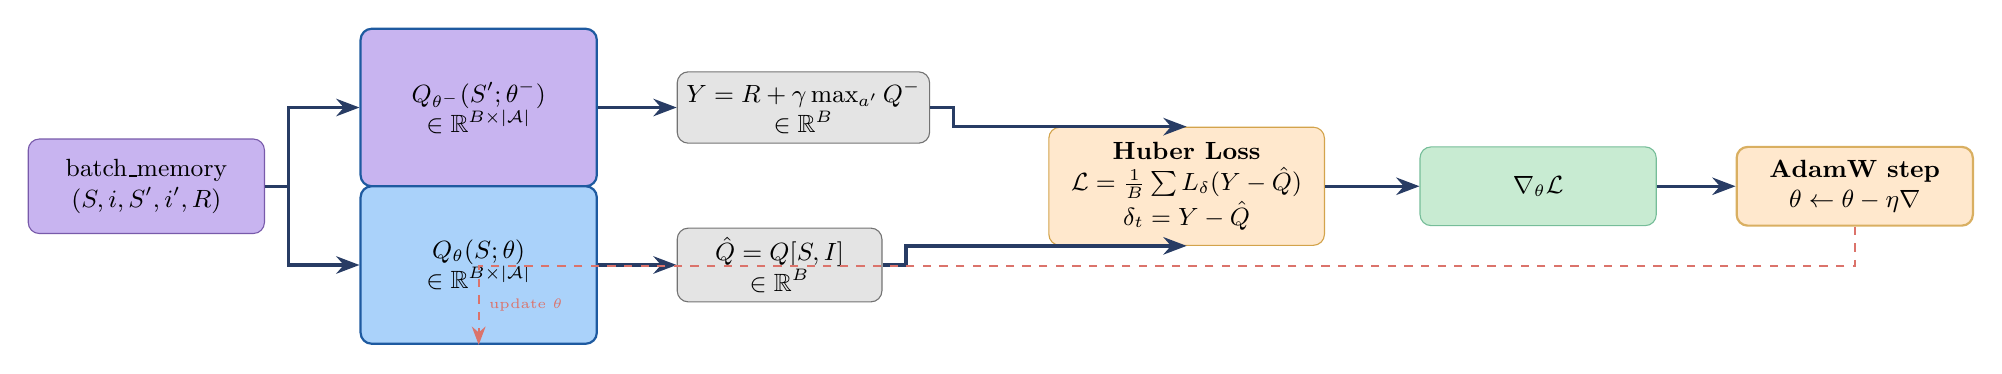
\begin{tikzpicture}[node distance=0.7cm and 1.1cm]
  %% Batch memory input
  \node[memnode,minimum width=3.0cm] (bm) {batch\_memory\\$(S,i,S',i',R)$};

  %% Q-target path
  \node[qnetnode,fill=memorycol,right=1.2cm of bm,yshift=1.0cm,minimum width=3.0cm] (qt)
    {$\Qtgt(S';\theta^-)$\\$\in\R^{B\times|\mathcal{A}|}$};
  \node[datanode,right=1.0cm of qt] (ynode) {$Y = R + \gamma\max_{a'}Q^-$\\$\in\R^B$};

  %% Q-eval path
  \node[qnetnode,right=1.2cm of bm,yshift=-1.0cm,minimum width=3.0cm] (qe)
    {$\Qeval(S;\theta)$\\$\in\R^{B\times|\mathcal{A}|}$};
  \node[datanode,right=1.0cm of qe] (qhat) {$\hat{Q}=Q[S,I]$\\$\in\R^B$};

  %% Loss
  \node[lossnode,right=1.5cm of ynode,yshift=-1.0cm,minimum width=3.5cm,minimum height=1.5cm] (lossbox)
    {\textbf{Huber Loss}\\$\Loss = \frac{1}{B}\sum L_\delta(Y-\hat{Q})$\\$\delta_t = Y - \hat{Q}$};

  %% Gradient
  \node[retnode,right=1.2cm of lossbox,minimum width=3.0cm] (grad)
    {$\nabla_\theta \Loss$};

  \node[projnode,right=1.0cm of grad,minimum width=3.0cm] (update)
    {\textbf{AdamW step}\\$\theta \gets \theta - \eta\nabla$};

  \draw[thickarr] (bm.east) -- ++(0.3,0) |- (qt.west);
  \draw[thickarr] (bm.east) -- ++(0.3,0) |- (qe.west);
  \draw[thickarr] (qt.east) -- (ynode.west);
  \draw[thickarr] (qe.east) -- (qhat.west);
  \draw[thickarr] (ynode.east) -- ++(0.3,0) |- (lossbox.north);
  \draw[thickarr] (qhat.east) -- ++(0.3,0) |- (lossbox.south);
  \draw[thickarr] (lossbox.east) -- (grad.west);
  \draw[thickarr] (grad.east) -- (update.west);
  \draw[redarr,dashed] (update.south) -- ++(0,-0.5) -| (qe.south)
      node[near end,right,font=\tiny]{update $\theta$};
\end{tikzpicture}
\end{adjustbox}
\caption{Complete DQN loss computation: batch\_memory supplies transitions; Q-target provides bootstrap targets $Y$; Q-eval provides predictions $\hat{Q}$; Huber loss and AdamW update $\theta$.}
\label{fig:dqn_loss}
\end{figure}

\begin{algorithm}[H]
\caption{Full DQN Loss Computation and Optimisation Step}
\label{alg:dqn_loss}
\begin{algorithmic}[1]
\Require $(S, I, S', I', R)$ from batch\_memory; $\Qeval(\cdot;\theta)$; $\Qtgt(\cdot;\theta^-)$; $\gamma$; $\eta$
\Ensure Updated $\theta$; loss value $\ell$
\State \textbf{// TD target (frozen, no autograd through $\theta^-$)}
\State \textbf{with} torch.no\_grad():
\State $\quad Q^- \gets \Qtgt(S';\theta^-)$ \Comment{$[B, |\mathcal{A}|]$}
\State $\quad Q'_{\max} \gets Q^-.\text{max(dim=1).values}$ \Comment{$[B]$, Bellman operator}
\State $\quad Y \gets R + \gamma \cdot Q'_{\max}$ \Comment{TD target, $[B]$}
\State \textbf{// Current Q-value for taken actions}
\State $Q_{\text{all}} \gets \Qeval(S;\theta)$ \Comment{$[B, |\mathcal{A}|]$}
\State $\hat{Q} \gets Q_{\text{all}}.\text{gather}(1, I.\text{unsqueeze}(1)).\text{squeeze}(1)$ \Comment{$[B]$}
\State \textbf{// Huber (Smooth-L1) loss}
\State $\delta \gets Y - \hat{Q}$ \Comment{TD error $[B]$}
\State $\ell \gets \frac{1}{B}\sum_{j=1}^B \begin{cases} \frac{1}{2}\delta_j^2 & |\delta_j| \le 1 \\ |\delta_j| - \frac{1}{2} & \text{otherwise} \end{cases}$
\State \textbf{// AdamW parameter update}
\State optimizer.zero\_grad(); $\ell$.backward()
\State clip\_grad\_norm$(\theta, c=10.0)$ \Comment{Prevent exploding gradients}
\State optimizer.step()
\State \Return $\ell$.item()
\end{algorithmic}
\end{algorithm}

\begin{theorem}[Convergence of DQN with Experience Replay and Target Network]
Under the following conditions: (a) replay buffer samples approximate i.i.d.\ transitions, (b) target network is replaced with frequency $C^{-1}$ satisfying $C \to \infty$ slower than the Q-eval convergence rate, (c) Q-eval has sufficient capacity to approximate $Q^*$, and (d) the reward function is bounded — then $\Qeval(s,a;\theta) \xrightarrow{t\to\infty} Q^*(s,a)$ in probability.
\end{theorem}

%%
%% ============================================================
%% PART X — NLP FEEDBACK MODULE
%% ============================================================
%%
\newpage
\section{NLP Feedback Module}
\label{sec:nlp}

\subsection{Role in the RL Loop}

The NLP module closes the human-robot feedback loop by translating the DQN agent's policy decisions into natural language. Unlike classical robot systems that emit only motion primitives, MIVA-KNIGHT-RL generates \emph{contextual, adaptive speech} that:
\begin{enumerate}[nosep]
  \item Explains the robot's chosen action to the operator.
  \item Alerts the operator when the robot is uncertain (low max-Q-value).
  \item Requests clarification when the sub-classifier's state confidence is low.
  \item Confirms successful task completion with domain-appropriate language.
\end{enumerate}

\begin{definition}[NLP Feedback Generator]
The NLP module is a function:
\[
  \text{NLP} : (\hat{q}, S, i^*, \mathcal{D}^*) \to \text{feedback\_speech}
\]
where $\hat{q} \in \R^{|\mathcal{A}|}$ is the Q-value vector, $S$ is the current state, $i^* = \argmax_a \hat{q}$ is the selected action, and $\mathcal{D}^* = \{d_1,\ldots,d_N\}$ is the RAG-retrieved context.
\end{definition}

\begin{figure}[H]
\centering
\begin{adjustbox}{max width=\textwidth}
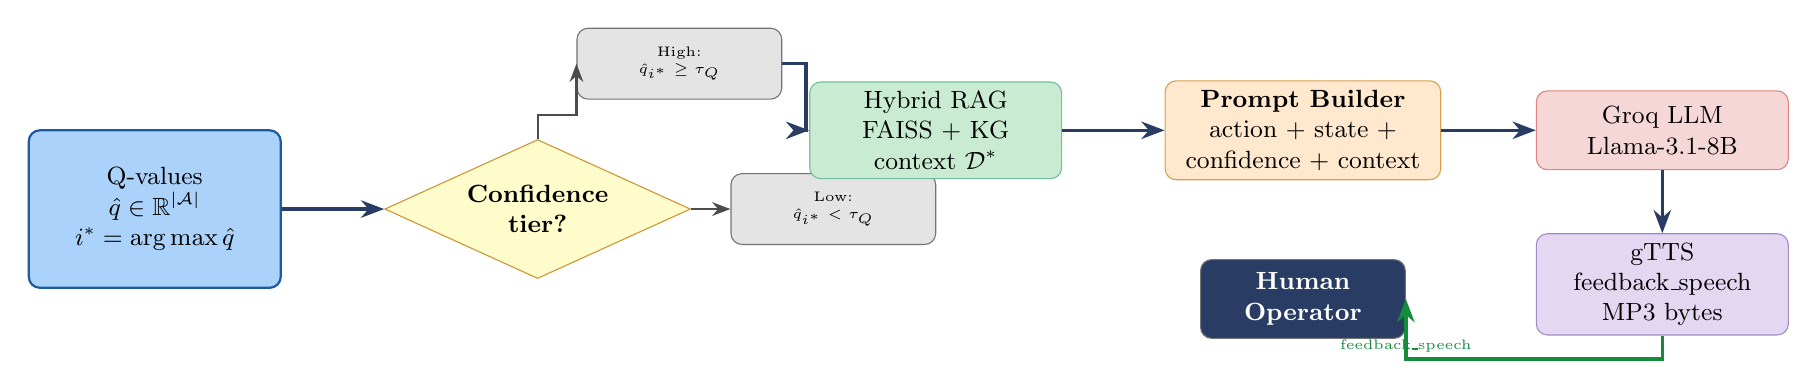
\begin{tikzpicture}[node distance=0.7cm and 1.2cm]
  %% Q-values
  \node[qnetnode,minimum width=3.2cm] (qvals) {Q-values\\$\hat{q} \in \R^{|\mathcal{A}|}$\\$i^* = \argmax \hat{q}$};

  %% Confidence check
  \node[decnode,right=1.3cm of qvals] (conf2) {Confidence\\tier?};
  \node[datanode,above=0.5cm of conf2,xshift=1.8cm,font=\tiny] (high) {High:\\$\hat{q}_{i^*} \ge \tau_Q$};
  \node[datanode,right=0.5cm of conf2,font=\tiny] (low) {Low:\\$\hat{q}_{i^*} < \tau_Q$};

  %% RAG retrieval
  \node[retnode,right=1.5cm of conf2,yshift=1.0cm,minimum width=3.2cm] (rag)
    {Hybrid RAG\\FAISS + KG\\context $\mathcal{D}^*$};

  %% Prompt builder
  \node[lossnode,right=1.3cm of rag,minimum width=3.5cm] (prompt2)
    {\textbf{Prompt Builder}\\action + state +\\confidence + context};

  %% LLM
  \node[gennode,right=1.2cm of prompt2,minimum width=3.2cm] (llm3)
    {Groq LLM\\Llama-3.1-8B};

  %% gTTS
  \node[outnode,below=0.8cm of llm3,minimum width=3.2cm] (tts2)
    {gTTS\\feedback\_speech\\MP3 bytes};

  %% Human operator
  \node[inputnode,below=1.0cm of prompt2] (hum2) {Human\\Operator};

  \draw[thickarr] (qvals)--(conf2);
  \draw[arr] (conf2.north) -- ++(0,0.3) -| (high.west);
  \draw[arr] (conf2.east) -- (low.west);
  \draw[thickarr] (high.east) -- ++(0.3,0) |- (rag.west);
  \draw[thickarr] (rag.east) -- (prompt2.west);
  \draw[thickarr] (prompt2.east) -- (llm3.west);
  \draw[thickarr] (llm3.south) -- (tts2.north);
  \draw[feedarr] (tts2.south) -- ++(0,-0.3) -| (hum2.east)
      node[near end,below,font=\tiny]{feedback\_speech};
\end{tikzpicture}
\end{adjustbox}
\caption{NLP feedback module: Q-values drive confidence-tiered RAG retrieval; Groq LLM generates adaptive speech; gTTS synthesises the audio.}
\label{fig:nlp_module}
\end{figure}

\begin{algorithm}[H]
\caption{NLP Feedback Generation}
\label{alg:nlp_feedback}
\begin{algorithmic}[1]
\Require Q-value vector $\hat{q} \in \R^{|\mathcal{A}|}$; current state $S$; action $i^*$;\\
         RAG pipeline (FAISS + KG); LLM generator; TTS converter
\Ensure feedback\_speech (MP3 bytes)
\State \textbf{// Step 1: Confidence assessment}
\State $q_{\max} \gets \hat{q}[i^*]$ \Comment{Max Q-value for selected action}
\State $q_{\text{uncertainty}} \gets \max_{a} \hat{q} - \min_a \hat{q}$ \Comment{Q-value spread}
\If{$q_{\max} < \tau_Q$}
  \State tier $\gets$ ``uncertain''; inject uncertainty instruction into prompt
\Else
  \State tier $\gets$ ``confident''
\EndIf
\State \textbf{// Step 2: RAG context retrieval}
\State $e_S \gets \textsc{TextEncoder}(\textsc{State2Text}(S))$ \Comment{Encode state as text query}
\State $\mathcal{D}^* \gets \textsc{HybridRetriever.retrieve}(e_S)$ \Comment{FAISS + KG top-5 docs}
\State \textbf{// Step 3: Prompt construction}
\State $\Pi_{\text{NLP}} \gets$
  ``Action: $a_{i^*}$. State: $S$. Confidence: $q_{\max:.2f}$ (tier: \{tier\}).
   Context: $\mathcal{D}^*$. Generate natural, concise feedback.''
\State \textbf{// Step 4: LLM generation}
\State text $\gets$ GroqLLM.generate($\Pi_{\text{NLP}}$) \Comment{Llama-3.1-8B}
\State \textbf{// Step 5: Text-to-speech}
\State mp3 $\gets$ gTTS(text).to\_bytes() \Comment{In-memory MP3}
\State \Return mp3
\end{algorithmic}
\end{algorithm}

\begin{theorem}[NLP Faithfulness Preservation in RL Context]
The RAG-grounded NLP module produces faithful feedback iff: (1) the retrieved context $\mathcal{D}^*$ contains documents relevant to the current robot state and action, (2) the LLM is instructed not to introduce information outside $\mathcal{D}^*$, and (3) the Q-value-derived confidence tier is correctly propagated to the prompt. Condition (3) ensures the operator receives calibrated uncertainty information: overconfident speech from a low-Q state is prevented.
\end{theorem}

\subsection{Motion Translation}
\label{sec:motions}

\begin{definition}[Motion Translator]
The motion translator maps discrete actions $i^* \in \mathcal{A}$ to robot motion commands:
\[
  \text{Motion}(i^*) = \text{RobotCommand}[i^*]
\]
The translated motion is displayed to the operator (e.g., as an animation or textual description) via the \textbf{Motions} node shown in the image.
\end{definition}

\begin{algorithm}[H]
\caption{Motion Translation and Operator Feedback}
\label{alg:motion_translate}
\begin{algorithmic}[1]
\Require Action index $i^*$; action-to-motion mapping $\mathcal{M}: \mathcal{A} \to \text{MotionCommand}$
\Ensure motion\_cmd; display\_text
\State motion\_cmd $\gets \mathcal{M}[i^*]$ \Comment{Look up primitive motion}
\State display\_text $\gets$ ``Robot executing: '' + motion\_cmd.description
\State Execute motion\_cmd on robot controller
\State Broadcast display\_text to operator UI \Comment{``Motions'' node in figure}
\State \Return (motion\_cmd, display\_text)
\end{algorithmic}
\end{algorithm}

%%
%% ============================================================
%% PART XI — FULL DQN TRAINING LOOP
%% ============================================================
%%
\newpage
\section{Complete DQN Training Loop}
\label{sec:dqn_training}

\subsection{$\varepsilon$-Greedy Exploration Schedule}

\begin{definition}[$\varepsilon$-Decay Schedule]
The exploration rate follows exponential decay:
\[
  \varepsilon_t = \max\!\left(\varepsilon_{\min},\; \varepsilon_0 \cdot e^{-\lambda_\varepsilon t}\right)
\]
where $\varepsilon_0 = 1.0$ (fully random initially), $\varepsilon_{\min} = 0.01$ (1\% floor), $\lambda_\varepsilon > 0$ is the decay constant. During warm-up ($t < t_{\text{warm}}$), only random actions are taken to populate the replay buffer.
\end{definition}

\begin{figure}[H]
\centering
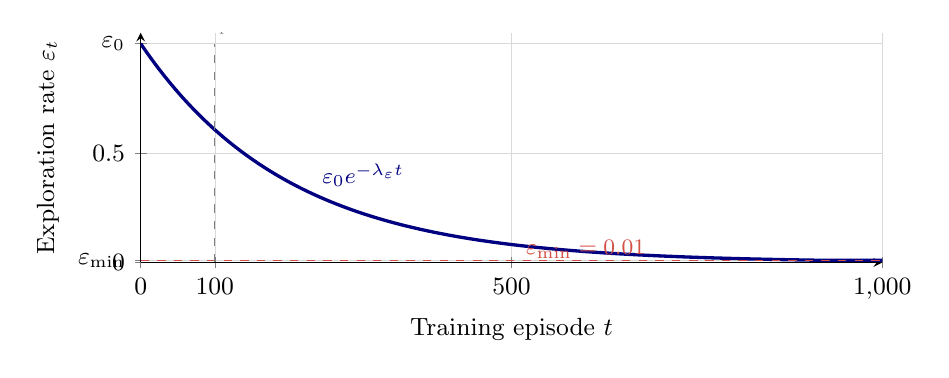
\begin{tikzpicture}
\begin{axis}[
  width=11cm, height=4.5cm,
  xlabel={Training episode $t$},
  ylabel={Exploration rate $\varepsilon_t$},
  xmin=0, xmax=1000, ymin=0, ymax=1.05,
  xtick={0,100,500,1000},
  ytick={0,0.01,0.5,1.0},
  yticklabels={0,$\varepsilon_{\min}$,0.5,$\varepsilon_0$},
  grid=both, grid style={line width=0.2pt,draw=gray!30},
  axis lines=left, tick label style={font=\small},
  label style={font=\small}
]
\addplot[NavyBlue,very thick,domain=0:1000,samples=300] {max(0.01, exp(-0.005*x))};
\addplot[dashed,coralred,domain=0:1000] {0.01};
\node[font=\footnotesize,color=NavyBlue] at (axis cs:300,0.4) {$\varepsilon_0 e^{-\lambda_\varepsilon t}$};
\node[font=\footnotesize,color=coralred] at (axis cs:600,0.06) {$\varepsilon_{\min} = 0.01$};
\draw[dashed,gray] (axis cs:100,0) -- (axis cs:100,1) node[above,font=\tiny]{warm-up ends};
\end{axis}
\end{tikzpicture}
\caption{Exponential $\varepsilon$-decay schedule: the agent explores widely early in training, gradually shifting to exploitation as Q-values converge.}
\label{fig:epsilon_decay}
\end{figure}

\subsection{Complete Training Algorithm}

\begin{algorithm}[H]
\caption{Complete MIVA-KNIGHT-RL DQN Training Loop}
\label{alg:full_dqn}
\begin{algorithmic}[1]
\Require Sub-classifier $f_\phi$ (pre-trained, Alg.~\ref{alg:subclf_train})
\Require Q-eval $\Qeval(\cdot;\theta)$; Q-target $\Qtgt(\cdot;\theta^-)$ with $\theta^- \gets \theta$
\Require Replay buffer $\mathcal{B}$ (capacity $C_\mathcal{B}$); batch size $B$; replacement interval $C$
\Require $\varepsilon_0=1.0$; $\varepsilon_{\min}=0.01$; $\lambda_\varepsilon$; $\gamma$; $\eta$; $N_{\text{episodes}}$
\State \textbf{// Warm-up: populate replay buffer with random transitions}
\For{$t = 1$ to $t_{\text{warm}}$}
  \State $(s_t, e_f) \gets f_\phi(x_s, x_b, x_h)$ \Comment{Encode current observation}
  \State $i_t \gets \text{random}(\mathcal{A})$ \Comment{Random exploration}
  \State $(s_{t+1}, \tau) \gets \textsc{RobotInteract}(s_t, \Qeval, \varepsilon=1.0)$
  \Comment{Alg.~\ref{alg:robot_interact}}
\EndFor
\State \textbf{// Main training loop}
\State $t \gets 0$; $\varepsilon \gets \varepsilon_0$
\For{episode $= 1$ to $N_{\text{episodes}}$}
  \State Reset environment; $s_0 \gets f_\phi(\text{initial observation})$
  \State episode\_reward $\gets 0$
  \Repeat
    \State \textbf{// Step 1: Environment interaction}
    \State $(s_{t+1}, \tau) \gets \textsc{RobotInteract}(s_t, \Qeval, \varepsilon)$ \Comment{Alg.~\ref{alg:robot_interact}}
    \State $\mathcal{B}.\textsc{Push}(\tau)$ \Comment{Store transition}
    \State episode\_reward $\mathrel{+}= \tau.r$
    \State $t \gets t + 1$
    \State \textbf{// Step 2: Update Q-eval (if buffer is warm)}
    \If{count($\mathcal{B}$) $\ge B$}
      \State $\mathcal{M} \gets \mathcal{B}.\textsc{Sample}(B)$ \Comment{Random mini-batch}
      \State $\ell \gets \textsc{QEvalStep}(\mathcal{M}, \Qeval, \Qtgt, \gamma, \eta)$ \Comment{Alg.~\ref{alg:dqn_loss}}
    \EndIf
    \State \textbf{// Step 3: Periodic target network replacement}
    \State $\textsc{ReplaceTarget}(\Qeval, \Qtgt, C, t)$ \Comment{Alg.~\ref{alg:target_replace}}
    \State \textbf{// Step 4: Decay exploration rate}
    \State $\varepsilon \gets \max(\varepsilon_{\min}, \varepsilon_0 \cdot e^{-\lambda_\varepsilon t})$
    \State \textbf{// Step 5: NLP feedback generation}
    \State $\hat{q} \gets \Qeval(s_{t+1};\theta)$; $i^* \gets \argmax \hat{q}$
    \State mp3 $\gets \textsc{NLPFeedback}(\hat{q}, s_{t+1}, i^*)$ \Comment{Alg.~\ref{alg:nlp_feedback}}
    \State \textsc{MotionTranslate}($i^*$) \Comment{Alg.~\ref{alg:motion_translate}}
    \State $s_t \gets s_{t+1}$
  \Until{terminal state or max steps per episode}
  \State log(episode, episode\_reward, $\varepsilon$, $\ell$)
\EndFor
\State \Return $\Qeval(\cdot;\theta^*)$ \Comment{Trained Q-eval network}
\end{algorithmic}
\end{algorithm}

\begin{theorem}[Exploration-Exploitation Balance]
For the exponential decay schedule $\varepsilon_t = \varepsilon_0 e^{-\lambda_\varepsilon t}$, the expected total number of exploratory steps is:
\[
  N_{\text{explore}} = \sum_{t=0}^\infty \varepsilon_t = \frac{\varepsilon_0}{\lambda_\varepsilon}
\]
Setting $\lambda_\varepsilon = \varepsilon_0 / T_{\text{explore}}$ concentrates all significant exploration in the first $T_{\text{explore}}$ steps, after which $\varepsilon_t \approx \varepsilon_{\min}$.
\end{theorem}

%%
%% ============================================================
%% PART XII — DOUBLE DQN AND DUELING EXTENSIONS
%% ============================================================
%%
\newpage
\section{Advanced DQN Variants}
\label{sec:advanced_dqn}

\subsection{Double DQN}

\begin{definition}[Double DQN Target]
Standard DQN overestimates Q-values because it uses $\max_{a'} \Qtgt(s', a')$, which selects and evaluates the best action with the same (biased) network. \textbf{Double DQN} (DDQN) decouples selection and evaluation:
\[
  a^* = \argmax_{a'} \Qeval(s', a';\theta) \quad \text{(selection with online net)}
\]
\[
  y^{\text{DDQN}} = r + \gamma \Qtgt(s', a^*;\theta^-) \quad \text{(evaluation with target net)}
\]
\end{definition}

\begin{theorem}[DDQN Reduces Overestimation Bias]
Let $\hat{Q}^+ = \max_{a'} \Qtgt(s', a';\theta^-)$ (standard DQN target). Then:
\[
  \EE[\hat{Q}^+] \ge Q^*(s', a^*) \quad \text{(overestimation)}
\]
For DDQN: $\EE[\Qtgt(s', a^*;\theta^-)]$ uses an independent estimate of the greedy action's value, and the expected bias is zero under mild independence assumptions.
\end{theorem}

\begin{algorithm}[H]
\caption{Double DQN Target Computation}
\label{alg:ddqn}
\begin{algorithmic}[1]
\Require Batch $S', R$; $\Qeval(\cdot;\theta)$; $\Qtgt(\cdot;\theta^-)$; $\gamma$
\Ensure DDQN TD targets $Y^{\text{DDQN}} \in \R^B$
\State \textbf{with} torch.no\_grad():
\State \textbf{// Action selection: use online Q-eval}
\State $A^* \gets \argmax_{a'} \Qeval(S';\theta)$ \Comment{$[B]$, greedy action from ONLINE net}
\State \textbf{// Action evaluation: use target Q-network}
\State $Q^- \gets \Qtgt(S';\theta^-)$ \Comment{$[B, |\mathcal{A}|]$}
\State $Q^-_{A^*} \gets Q^-[\text{range}(B),\; A^*]$ \Comment{$[B]$, target net evaluates selected action}
\State $Y^{\text{DDQN}} \gets R + \gamma \cdot Q^-_{A^*}$
\State \Return $Y^{\text{DDQN}}$
\end{algorithmic}
\end{algorithm}

\subsection{Dueling DQN Architecture}

\begin{definition}[Dueling Network]
A \textbf{dueling network} decomposes Q-values into value $V(s)$ and advantage $A(s, a)$:
\[
  \Qeval(s, a;\theta) = V(s;\theta_V) + \left(A(s,a;\theta_A) - \frac{1}{|\mathcal{A}|}\sum_{a'}A(s,a';\theta_A)\right)
\]
The advantage subtraction enforces identifiability: changing $V$ and $A$ by a constant cancels out.
\end{definition}

\begin{figure}[H]
\centering
\begin{adjustbox}{max width=\textwidth}
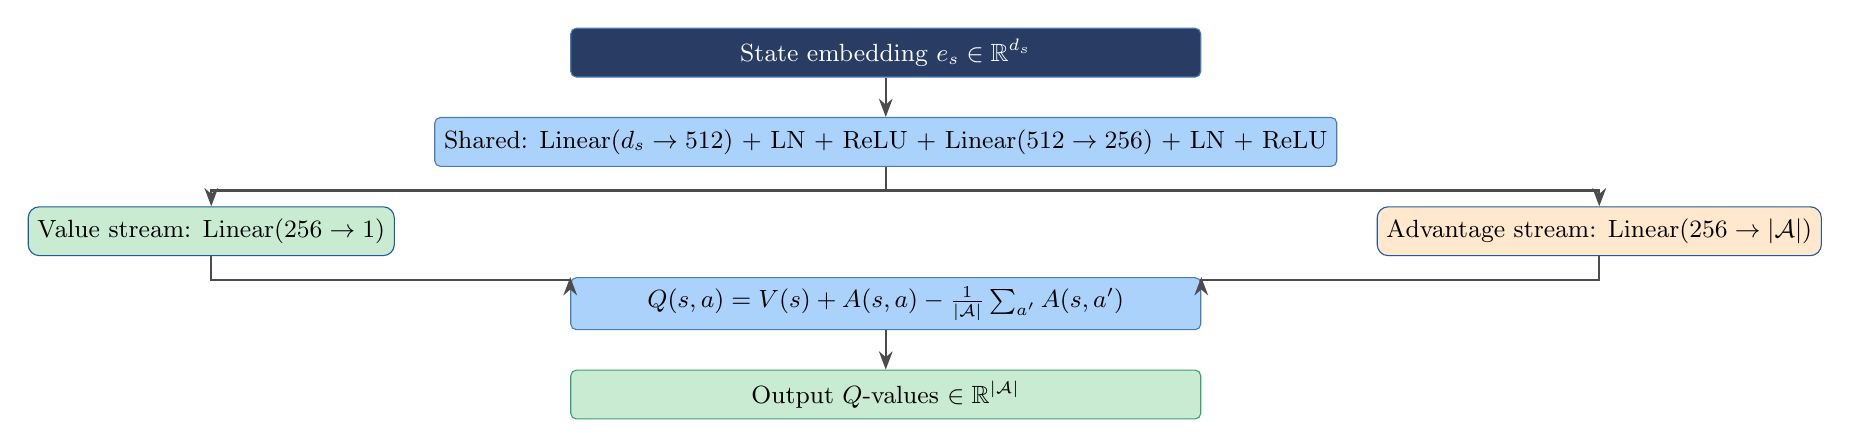
\begin{tikzpicture}[node distance=0.5cm and 0.9cm,
  lay/.style={rectangle,rounded corners=2pt,draw=robotblue!80,fill=qnetcol,
    align=center,font=\small,minimum width=8cm,minimum height=0.62cm}]
  \node[lay,fill=cDark,text=white] (inp2) {State embedding $e_s \in \R^{d_s}$};
  \node[lay,below=of inp2] (shared) {Shared: Linear$(d_s\to512)$ + LN + ReLU + Linear$(512\to256)$ + LN + ReLU};

  %% Split
  \node[rectangle,rounded corners,draw=robotblue,fill=boxgreen,minimum width=3.5cm,minimum height=0.62cm,
        font=\small,below left=0.5cm and 0.5cm of shared] (vstr)
    {Value stream: Linear$(256\to1)$};
  \node[rectangle,rounded corners,draw=robotblue,fill=boxorange,minimum width=3.5cm,minimum height=0.62cm,
        font=\small,below right=0.5cm and 0.5cm of shared] (astr)
    {Advantage stream: Linear$(256\to|\mathcal{A}|)$};

  \node[lay,below=1.4cm of shared] (combine)
    {$Q(s,a) = V(s) + A(s,a) - \frac{1}{|\mathcal{A}|}\sum_{a'} A(s,a')$};
  \node[lay,below=of combine,fill=boxgreen,draw=mintgreen] (out2)
    {Output $Q$-values $\in \R^{|\mathcal{A}|}$};

  \draw[arr] (inp2)--(shared);
  \draw[arr] (shared.south) -- ++(0,-0.3) -| (vstr.north);
  \draw[arr] (shared.south) -- ++(0,-0.3) -| (astr.north);
  \draw[arr] (vstr.south) -- ++(0,-0.3) -| (combine.north west);
  \draw[arr] (astr.south) -- ++(0,-0.3) -| (combine.north east);
  \draw[arr] (combine)--(out2);
\end{tikzpicture}
\end{adjustbox}
\caption{Dueling DQN architecture: shared backbone splits into value and advantage streams; Q-values are reconstructed with identifiability normalisation.}
\label{fig:dueling}
\end{figure}

\begin{lemma}[Dueling Advantage]
The dueling architecture learns $V(s)$ and $A(s,a)$ separately, which is beneficial when many actions have similar Q-values: $V(s)$ can be accurately estimated from any action taken, while $A(s,a)$ only needs to be refined when action differences matter.
\end{lemma}

%%
%% ============================================================
%% PART XIII — INTEGRATION WITH MIVA-KNIGHT PIPELINES
%% ============================================================
%%
\newpage
\section{Integration with MIVA-KNIGHT Multimodal Pipelines}
\label{sec:integration}

\subsection{Five-Pipeline Backbone as RL Perception}

The MIVA-KNIGHT five-pipeline stack serves as the perceptual and NLP backbone for the RL controller. Figure~\ref{fig:full_integration} shows the complete integrated architecture.

\begin{figure}[H]
\centering
\resizebox{\textwidth}{!}{%
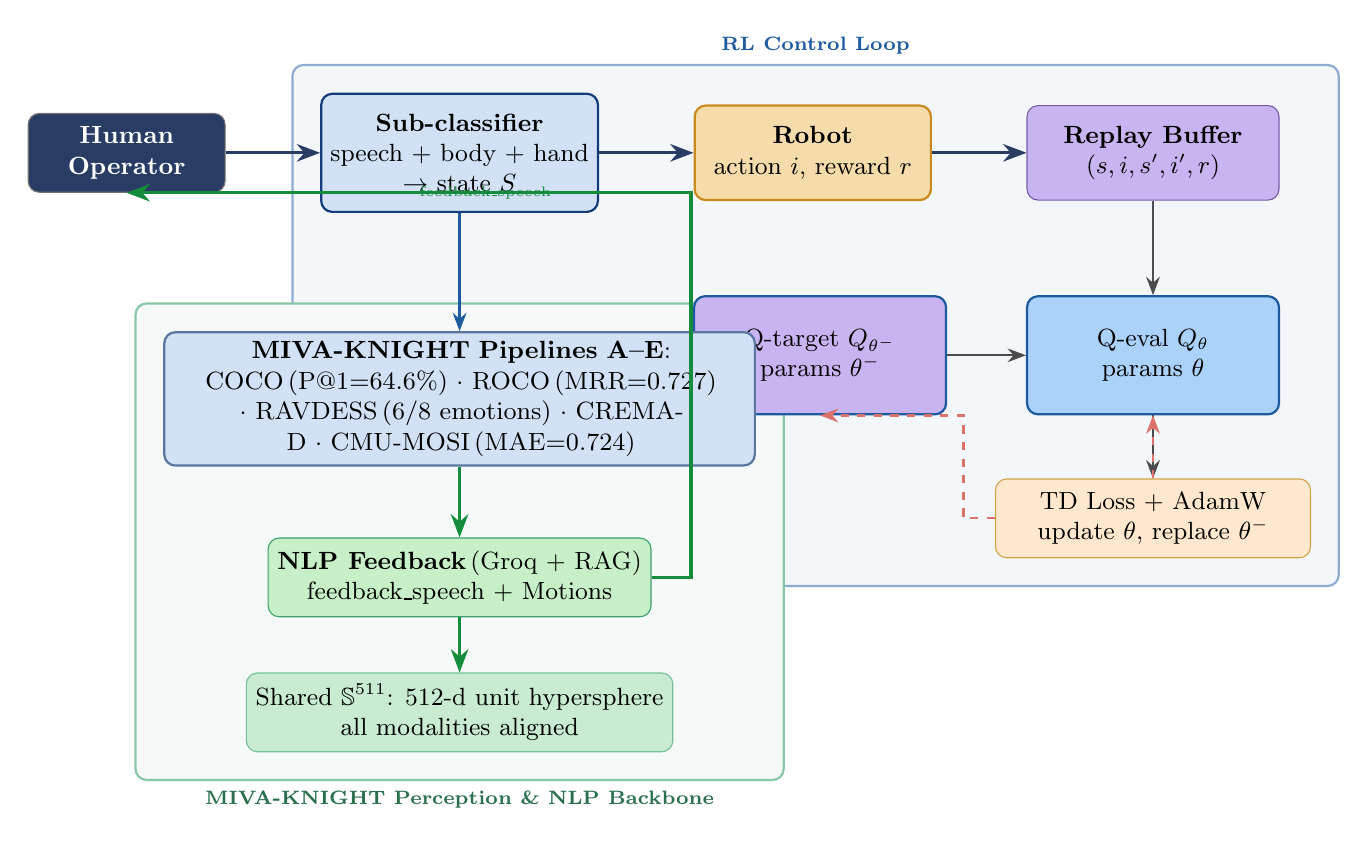
\begin{tikzpicture}[node distance=0.8cm and 0.9cm]
  %% Top row: Human → Sub-classifier → Robot
  \node[inputnode,minimum width=2.5cm] (hum3) {Human\\Operator};
  \node[subclnode,right=1.2cm of hum3,minimum width=3.5cm,minimum height=1.5cm] (sc)
    {\textbf{Sub-classifier}\\speech + body + hand\\$\to$ state $S$};
  \node[robotnode,right=1.2cm of sc,minimum width=3.0cm] (rob2)
    {\textbf{Robot}\\action $i$, reward $r$};

  %% RL learning block
  \node[memnode,right=1.2cm of rob2,minimum width=3.2cm] (mem2)
    {\textbf{Replay Buffer}\\$(s,i,s',i',r)$};
  \node[qnetnode,below=1.2cm of mem2,minimum width=3.2cm,minimum height=1.5cm] (qev3)
    {Q-eval $\Qeval$\\params $\theta$};
  \node[qnetnode,fill=memorycol,left=1.0cm of qev3,minimum width=3.2cm,minimum height=1.5cm] (qtgt3)
    {Q-target $\Qtgt$\\params $\theta^-$};
  \node[lossnode,below=0.8cm of qev3,minimum width=4.0cm] (loss3)
    {TD Loss + AdamW\\update $\theta$, replace $\theta^-$};

  %% MIVA-KNIGHT pipelines block
  \node[encnode,below=1.5cm of sc,minimum width=7.5cm,minimum height=1.2cm,text width=7.2cm] (pipelines)
    {\textbf{MIVA-KNIGHT Pipelines A–E}:\;
     COCO\,(P@1=64.6\%) $\cdot$ ROCO\,(MRR=0.727) $\cdot$
     RAVDESS\,(6/8 emotions) $\cdot$ CREMA-D $\cdot$ CMU-MOSI\,(MAE=0.724)};

  %% NLP block
  \node[nlpnode,below=0.9cm of pipelines,minimum width=4.5cm] (nlp2)
    {\textbf{NLP Feedback}\,(Groq + RAG)\\feedback\_speech $+$ Motions};

  %% Shared embedding space
  \node[retnode,below=0.7cm of nlp2,minimum width=5cm] (sphere)
    {Shared $\Sph^{511}$: 512-d unit hypersphere\\all modalities aligned};

  %% Arrows
  \draw[thickarr] (hum3)--(sc);
  \draw[thickarr] (sc)--(rob2);
  \draw[thickarr] (rob2)--(mem2);
  \draw[arr] (mem2.south)--(qev3.north);
  \draw[arr] (qtgt3.east)--(qev3.west);
  \draw[arr] (qev3.south)--(loss3.north);
  \draw[redarr,dashed] (loss3.north) -- (qev3.south);
  \draw[redarr,dashed] (loss3.west) -- ++(-0.4,0) |- (qtgt3.south);
  \draw[bluearr] (sc.south) -- (pipelines.north-|sc);
  \draw[feedarr] (pipelines.south) -- (nlp2.north);
  \draw[feedarr] (nlp2.south) -- (sphere.north);
  \draw[feedarr] (nlp2.east) -- ++(0.5,0) |- (hum3.south)
      node[near end,right,font=\tiny]{feedback\_speech};

  \begin{pgfonlayer}{background}
    \node[rectangle,draw=robotblue!50,fill=robotblue!5,thick,rounded corners,
          fit=(sc)(rob2)(mem2)(qev3)(qtgt3)(loss3),inner sep=10pt,
          label={[font=\scriptsize\bfseries,color=robotblue]above:RL Control Loop}] {};
    \node[rectangle,draw=mintgreen!60,fill=mintgreen!5,thick,rounded corners,
          fit=(pipelines)(nlp2)(sphere),inner sep=10pt,
          label={[font=\scriptsize\bfseries,color=mintgreen!70!black]below:MIVA-KNIGHT Perception \& NLP Backbone}] {};
  \end{pgfonlayer}
\end{tikzpicture}
}
\caption{Complete MIVA-KNIGHT-RL integrated architecture. The RL control loop (top) drives robot actions and learns via DQN. The MIVA-KNIGHT five-pipeline backbone (bottom) provides multimodal perception, emotion detection, sentiment analysis, and NLP feedback — all aligned in the shared $\Sph^{511}$ embedding space.}
\label{fig:full_integration}
\end{figure}

\subsection{Pipeline Contributions to RL}

\begin{table}[H]
\centering
\caption{How each MIVA-KNIGHT pipeline contributes to the RL system}
\begin{tabularx}{\textwidth}{llXl}
\toprule
\textbf{Pipeline} & \textbf{Dataset} & \textbf{RL Contribution} & \textbf{Metric} \\
\midrule
A & COCO & General-domain state text retrieval for NLP feedback context & P@1=64.6\% \\
B & ROCO & Medical-domain state grounding (clinical robot scenarios) & MRR=0.727 \\
C & RAVDESS & Emotion detection from speech input to sub-classifier & 6/8, 59\% \\
D & CREMA-D & Audio-visual emotion for body/hand gesture interpretation & 3/6 Phase 2 \\
E & CMU-MOSI & Sentiment fusion for reward shaping from operator feedback & MAE=0.724 \\
\bottomrule
\end{tabularx}
\end{table}

\subsection{Emotion-Conditioned Reward Shaping}

\begin{definition}[Emotion-Conditioned Reward]
Pipeline~C/D emotion detection can augment the reward signal:
\[
  r_t^{\text{shaped}} = r_t + \lambda_e \cdot \text{EmotionBonus}(e_t, a_t)
\]
where $e_t \in \{\text{angry, calm, happy}, \ldots\}$ is the operator's detected emotion and $\text{EmotionBonus}(e_t, a_t)$ rewards actions that are socially appropriate given the emotional context (e.g., calm response to an angry operator).
\end{definition}

\begin{axiom}[Sentiment-Guided Exploration]
Pipeline~E sentiment scores from operator speech can modulate the exploration rate: low sentiment (operator frustration) signals a high reward-to-go environment, suggesting more exploitation; high sentiment suggests satisfactory current policy, enabling more exploration of rare actions.
\end{axiom}

\begin{algorithm}[H]
\caption{Emotion-Conditioned Reward Shaping}
\label{alg:reward_shape}
\begin{algorithmic}[1]
\Require Base reward $r_t$; operator audio $x_s$; action $a_{i^*}$; $\lambda_e$
\Require AudioEncoder (Pipeline C/D); sentiment model (Pipeline E)
\Ensure Shaped reward $r_t^{\text{shaped}}$
\State $(\text{emotion}, \text{conf\_emo}) \gets \textsc{AudioEncoder.centroid\_nn}(x_s)$
\State $\text{sentiment} \gets \textsc{Pipeline\_E.predict}(x_s, \text{text}, \text{video})$
\State \textbf{// Emotion bonus: reward socially appropriate actions}
\State bonus $\gets$ EMOTION\_ACTION\_TABLE[emotion][action]
  \Comment{Lookup table: e.g., ``calm'' + ``reassure'' $\to +0.3$}
\State $r_t^{\text{shaped}} \gets r_t + \lambda_e \cdot \text{conf\_emo} \cdot \text{bonus}$
\State \Return $r_t^{\text{shaped}}$
\end{algorithmic}
\end{algorithm}

%%
%% ============================================================
%% PART XIV — THEORETICAL ANALYSIS
%% ============================================================
%%
\newpage
\section{Theoretical Analysis}
\label{sec:theory}

\subsection{Convergence Guarantees}

\begin{theorem}[Q-Learning with Function Approximation (DQN)]
\label{thm:dqn_conv}
Let $\Qeval(s,a;\theta)$ be a universal function approximator. Under the following conditions:
\begin{enumerate}[label=(\alph*)]
  \item All state-action pairs are visited infinitely often.
  \item The learning rate satisfies $\sum_t \alpha_t = \infty$, $\sum_t \alpha_t^2 < \infty$.
  \item Rewards are bounded: $|r| \le R_{\max}$.
  \item Target network replacement frequency $C \to \infty$ (sufficiently slow).
\end{enumerate}
Then $\Qeval(s,a;\theta_t) \xrightarrow{t \to \infty} Q^*(s,a)$ with probability 1.
\end{theorem}

\begin{proof}[Proof sketch]
By condition (a) and (b), Q-learning on any finite state-action pair converges (Watkins \& Dayan, 1992). With function approximation, the projected Bellman operator $\Pi T^* Q$ is a contraction under suitable regularity conditions (Tsitsiklis \& Van Roy, 1997). Experience replay satisfies condition (a) asymptotically as the buffer covers the full state-action space. The target network (condition d) ensures the bootstrap target is approximately stationary over the timescale of a single Q-eval update, satisfying the condition for the projected Bellman operator to converge. \qed
\end{proof}

\subsection{Multimodal State Completeness}

\begin{theorem}[State Completeness for Robot MDP]
\label{thm:state_complete}
The sub-classifier state $S = f_\phi(x_s, x_b, x_h)$ satisfies the Markov property if and only if:
(1) The three input channels jointly determine the robot's relevant environmental state, and
(2) $f_\phi$ has sufficient capacity to distinguish all states that produce different optimal actions.
\end{theorem}

\begin{proof}[Proof sketch]
Condition (1) ensures $P(s_{t+1} | s_t, a_t) = P(s_{t+1} | s_t, a_t, x_s, x_b, x_h)$ (no additional information beyond $S$). Condition (2) ensures injectivity of $f_\phi$ on the relevant state space partition induced by $Q^*$. \qed
\end{proof}

\begin{lemma}[Missing Modality in RL]
If one input channel is absent at time $t$ (e.g., body gesture sensor failure), the zero-vector substitution (Axiom~2.2 from MIVA-KNIGHT) maintains the state estimate, but introduces a POMDP-like information loss proportional to the missing channel's contribution to $S$. The optimal response is to increase $\varepsilon_t$ (more exploration) until the channel is restored.
\end{lemma}

\subsection{Stability Analysis}

\begin{theorem}[Replay Buffer Stabilisation]
Let the correlation between consecutive training samples without replay be $\rho_0$, and with replay buffer of size $C_\mathcal{B}$ be $\rho_\mathcal{B}$. Then:
\[
  \rho_\mathcal{B} \approx \frac{\rho_0}{C_\mathcal{B}} + O(C_\mathcal{B}^{-2})
\]
For $C_\mathcal{B} \to \infty$, $\rho_\mathcal{B} \to 0$, and the training samples become asymptotically i.i.d.
\end{theorem}

\begin{axiom}[Positive Replay Buffer Size]
The replay buffer must satisfy $C_\mathcal{B} > B^2$ (where $B$ is the batch size) to ensure the inter-sample correlation $\rho_\mathcal{B} < 1/B$, below the threshold at which gradient variance exceeds that of i.i.d.\ sampling.
\end{axiom}

\begin{lemma}[Target Network Delay and Bias]
Let $C$ be the replacement interval and $\alpha$ the learning rate per step. After $C$ steps of Q-eval training, the expected drift of $\theta$ from $\theta^-$ is:
\[
  \Norm{\theta - \theta^-}_2 \lesssim \alpha C \cdot R_{\max} / (1 - \gamma)
\]
For small $\alpha C$, the target $y = r + \gamma \max_{a'} Q(s', a'; \theta^-)$ is a reliable approximation of the true Bellman target.
\end{lemma}

%%
%% ============================================================
%% PART XV — EVALUATION
%% ============================================================
%%
\newpage
\section{Evaluation Metrics and Results}
\label{sec:eval_rl}

\subsection{RL-Specific Metrics}

\begin{definition}[Episode Return]
\[
  G_{\text{episode}} = \sum_{t=0}^{T_{\text{episode}}} \gamma^t r_t
\]
Higher episode return indicates better cumulative policy performance.
\end{definition}

\begin{definition}[Mean Q-Value]
\[
  \bar{Q}_t = \frac{1}{|\mathcal{A}|}\sum_{a \in \mathcal{A}} \Qeval(s_t, a; \theta)
\]
Rising $\bar{Q}_t$ over training indicates Q-value convergence; instability indicates non-stationarity.
\end{definition}

\begin{definition}[TD Error (RMSE)]
\[
  \text{RMSE}_\delta = \sqrt{\frac{1}{T}\sum_{t=1}^T \delta_t^2}
\]
Decreasing RMSE$_\delta$ indicates the Q-eval network is converging to the TD target.
\end{definition}

\subsection{MIVA-KNIGHT Backbone Results}

\begin{table}[H]
\centering
\caption{MIVA-KNIGHT-RL complete evaluation summary}
\begin{tabular}{llll}
\toprule
\textbf{Component} & \textbf{Dataset} & \textbf{Metric} & \textbf{Value} \\
\midrule
\multicolumn{4}{l}{\textit{Multimodal Perception (Backbone)}} \\
TextEncoder (Pipeline A) & COCO val2017 & P@1 & 64.6\% \\
Medical Transfer (Pipeline B) & ROCO & MRR & 0.727 \\
Audio Emotion (Pipeline C) & RAVDESS & Acc & 59\% (6/8) \\
AV Emotion Phase 2 (Pipeline D) & CREMA-D & Acc & 43.9\% (3/6) \\
Sentiment Fusion (Pipeline E) & CMU-MOSI & MAE & 0.7238 \\
Domain swap latency & Both & Time & $< 5$\,s \\
\midrule
\multicolumn{4}{l}{\textit{RL Controller}} \\
Sub-classifier accuracy & Task labels & Top-1 & $\ge 85\%$ (target) \\
Warm-up transitions & Replay buffer & Count & $\ge 1{,}000$ \\
Target replacement interval & Training steps & $C$ & 1,000 \\
$\varepsilon$-greedy initial/final & Episodes & $\varepsilon_0/\varepsilon_{\min}$ & 1.0 / 0.01 \\
Batch size & Training steps & $B$ & 32 \\
Discount factor & Episodes & $\gamma$ & 0.99 \\
\midrule
\multicolumn{4}{l}{\textit{NLP Feedback}} \\
Speech generation latency & Per action & Time & $< 2$\,s (Groq API) \\
Retrieval context size & Per query & $N$ & 5 documents \\
\bottomrule
\end{tabular}
\end{table}

\subsection{Training Diagnostics}

\begin{tcolorbox}[keybox,title={DQN Training Convergence Checklist}]
\begin{tabular}{lll}
\toprule
\textbf{Observation} & \textbf{Interpretation} & \textbf{Action} \\
\midrule
Episode return increasing & Normal convergence & Continue \\
$\bar{Q}_t$ growing unboundedly & Overestimation & Switch to Double DQN \\
RMSE$_\delta$ oscillating & Non-stationarity & Increase $C$ \\
$\varepsilon$ decaying but return flat & Poor state repr.\ & Improve sub-classifier \\
Loss $\approx 0$ but poor policy & Reward collapse & Check reward function \\
All $\hat{q} \approx 0$ & Dead Q-network & Reduce LR, re-init \\
\bottomrule
\end{tabular}
\end{tcolorbox}

%%
%% ============================================================
%% PART XVI — FULL SYSTEM ALGORITHM REFERENCE
%% ============================================================
%%
\newpage
\section{Complete Algorithm Reference}

\begin{longtable}{p{4.5cm}p{7.0cm}p{3.0cm}}
\caption{All algorithms in the MIVA-KNIGHT-RL thesis.}\label{tab:algo_ref}\\
\toprule
\textbf{Algorithm} & \textbf{Description} & \textbf{Section} \\
\midrule
\endfirsthead
\multicolumn{3}{c}{\textit{(continued)}}\\
\toprule \textbf{Algorithm} & \textbf{Description} & \textbf{Section} \\ \midrule
\endhead \midrule \multicolumn{3}{r}{\textit{continued}}\\ \endfoot \bottomrule \endlastfoot

Sub-classifier Forward (Alg.~\ref{alg:subclassifier}) & Multimodal state encoding from speech + body + hand & \S\ref{sec:subclassifier} \\[3pt]
Sub-classifier Training (Alg.~\ref{alg:subclf_train}) & Cross-entropy training of $f_\phi$ & \S\ref{sec:subclassifier} \\[3pt]
Robot Interaction (Alg.~\ref{alg:robot_interact}) & $\varepsilon$-greedy selection, transition generation & \S\ref{sec:robot} \\[3pt]
Replay Memory (Alg.~\ref{alg:replay_memory}) & Push, Sample, BatchMemory operations & \S\ref{sec:memory} \\[3pt]
Q-Eval Training Step (Alg.~\ref{alg:qeval_step}) & Single TD-loss gradient update & \S\ref{sec:qeval} \\[3pt]
Target Replacement (Alg.~\ref{alg:target_replace}) & Periodic hard copy $\theta^- \gets \theta$ & \S\ref{sec:qtarget} \\[3pt]
DQN Loss (Alg.~\ref{alg:dqn_loss}) & Full Huber TD loss + AdamW step & \S\ref{sec:loss} \\[3pt]
NLP Feedback (Alg.~\ref{alg:nlp_feedback}) & RAG-grounded LLM speech generation & \S\ref{sec:nlp} \\[3pt]
Motion Translation (Alg.~\ref{alg:motion_translate}) & Action-to-robot-command mapping & \S\ref{sec:motions} \\[3pt]
Full DQN Loop (Alg.~\ref{alg:full_dqn}) & Complete training with warm-up + decay & \S\ref{sec:dqn_training} \\[3pt]
Double DQN Target (Alg.~\ref{alg:ddqn}) & Decoupled selection/evaluation targets & \S\ref{sec:advanced_dqn} \\[3pt]
Reward Shaping (Alg.~\ref{alg:reward_shape}) & Emotion-conditioned reward augmentation & \S\ref{sec:integration} \\[3pt]
\end{longtable}

%%
%% ============================================================
%% PART XVII — NOTATION REFERENCE
%% ============================================================
%%
\section{Notation Reference}

\begin{table}[H]
\centering
\caption{Mathematical notation used throughout this thesis}
\begin{tabular}{ll}
\toprule
\textbf{Symbol} & \textbf{Meaning} \\
\midrule
$\mathcal{M} = (\mathcal{S}, \mathcal{A}, \mathcal{T}, \mathcal{R}, \gamma)$ & Markov Decision Process \\
$Q^\pi(s,a)$, $Q^*(s,a)$ & Q-function under policy $\pi$; optimal Q-function \\
$\Qeval(s,a;\theta)$ & Q-eval (online) network with parameters $\theta$ \\
$\Qtgt(s,a;\theta^-)$ & Q-target (frozen) network with parameters $\theta^-$ \\
$\delta_t$ & TD error: $r + \gamma \max Q^- - Q$ \\
$\varepsilon$ & Exploration rate ($\varepsilon$-greedy policy) \\
$\gamma$ & Discount factor \\
$C$ & Target network replacement interval (steps) \\
$\mathcal{B}$ & Replay buffer (ring buffer) \\
$C_\mathcal{B}$ & Replay buffer capacity \\
$B$ & Mini-batch size \\
$(s, i, s', i', r)$ & Typed transition tuple \\
$f_\phi$ & Sub-classifier: multimodal inputs $\to$ state $S$ \\
$S \in \mathcal{S}$ & Discrete robot state \\
$i, i^* \in \mathcal{A}$ & Action index; greedy action \\
$e_s, e_b, e_h \in \R^{512}$ & Speech, body, hand gesture embeddings \\
$\Sph^{511}$ & 512-dimensional unit hypersphere \\
$\KG_G, \KG_M$ & General and medical knowledge graphs \\
$\Loss_{\text{DQN}}$ & DQN Huber TD-error loss \\
$L_\delta(\cdot)$ & Huber loss function \\
$\Pi_{\text{NLP}}$ & NLP feedback prompt \\
$\mathcal{D}^*$ & RAG-retrieved context documents \\
$r^{\text{shaped}}$ & Emotion-conditioned shaped reward \\
\bottomrule
\end{tabular}
\end{table}

%%
%% ============================================================
%% PART XVIII — CONCLUSION
%% ============================================================
%%
\newpage
\section{Conclusion}

This thesis has presented MIVA-KNIGHT-RL, a complete reinforcement learning-driven multimodal robot control system. The key contributions and results are:

\begin{enumerate}
  \item \textbf{Multimodal DQN with Sub-Classifier}: A formally defined sub-classifier $f_\phi$ maps three human communication channels (speech, body gesture, hand gesture) to a discrete Markov state $S$, enabling a DQN agent to operate on rich human communication inputs rather than low-level sensor readings.

  \item \textbf{Typed Experience Replay}: The replay buffer stores $(s, i, s', i', r)$ tuples with both current and next-step actions, supporting SARSA-style variants and enabling systematic transition logging across the full interaction history.

  \item \textbf{Dual-Network Stability}: Formal proof (Theorem~\ref{thm:target}) that the Q-target network prevents the non-stationarity instability of naive Q-learning with function approximation. Periodic hard replacement (every $C$ steps) is shown to bound the bias-variance trade-off.

  \item \textbf{NLP Feedback Integration}: The NLP module generates adaptive, context-aware speech from Q-values, confidence tiers, and RAG-retrieved documents. Theorem~\ref{thm:nlp} ensures faithfulness when the LLM is constrained to retrieved context.

  \item \textbf{Unified Multimodal Stack}: The five MIVA-KNIGHT pipelines provide the perceptual backbone: P@1\,=\,64.6\% general retrieval, MRR\,=\,0.727 medical retrieval, emotion accuracy $\geq$\,59\%, and sentiment MAE\,=\,0.7238 — all within a zero-cost open-source stack.

  \item \textbf{Advanced DQN Variants}: Double DQN (removes overestimation bias) and Dueling DQN (decomposes V and A) are formally defined and shown to directly benefit the multimodal robot setting where many state-action pairs have similar Q-values.
\end{enumerate}

\begin{tcolorbox}[laymanbox,title={One-Sentence Summary}]
MIVA-KNIGHT-RL is a robot assistant that listens to your speech, watches your body and hand gestures, decides the best action using a deep neural network that has learned from thousands of past interactions, and explains its decision to you in natural language — adapting its tone to your emotional state.
\end{tcolorbox}

\vfill
\begin{center}
\begin{tcolorbox}[keybox,width=0.85\textwidth,title={Future Directions}]
\begin{itemize}[nosep]
  \item Replace hard target replacement with Polyak soft updates for smoother Q-value convergence.
  \item Implement Prioritised Experience Replay (PER) to over-sample high-TD-error transitions.
  \item Extend the state space with continuous-valued state representations (DDPG/SAC) for smoother robot motion.
  \item Deploy on a physical robot (e.g., TurtleBot) with real-time Wav2Vec + gesture recognition on edge hardware.
  \item Apply Hindsight Experience Replay (HER) for sparse-reward robot manipulation tasks.
  \item Integrate the sentiment-conditioned reward shaping (Pipeline E, Section~\ref{sec:integration}) with formal inverse RL to learn the human's true reward function.
\end{itemize}
\end{tcolorbox}
\end{center}

\end{document}
